% presentation
\documentclass{beamer}
\usetheme[height=7mm]{Rochester}
\usecolortheme{rose}

% handout

%\documentclass[handout]{beamer}
%\usepackage{pgfpages} \pgfpagesuselayout{8 on 1}[a4paper]

%\documentclass[mathserif]{article}
%\usepackage{beamerarticle}

\usepackage{amsmath}
\usepackage{comment}
\usepackage{amssymb,amsfonts}
\usepackage[T1]{fontenc}
\usepackage{lmodern}
\usepackage{tikz}
\usepackage{simpsons}
\usepackage{marvosym}
\usepackage{color}
\usepackage{multirow}
\usepackage{pgffor}
\usepackage[slide,algoruled,titlenumbered,vlined,noend,linesnumbered,]{algorithm2e}

\usefonttheme{structurebold}

\setbeamertemplate{footline}[frame number]
\setbeamertemplate{navigation symbols}{}
\setbeamerfont{smallverb}{size*={73}}
\usefonttheme[onlymath]{serif}
\setbeamertemplate{theorems}[numbered]
\newtheorem{construction}[theorem]{Construction}
\newtheorem{proposition}[theorem]{Proposition}

\AtBeginSection[] { 
  \begin{frame} 
    \frametitle{Content} 
    \tableofcontents[currentsection]
  \end{frame} 
  \addtocounter{framenumber}{-1} 
}

\usetikzlibrary[shapes.arrows]
\usetikzlibrary{shapes.geometric}
\usetikzlibrary{backgrounds}
\usetikzlibrary{positioning}
\usetikzlibrary{calc}
\usetikzlibrary{intersections}
\usetikzlibrary{fadings}
\usetikzlibrary{decorations.footprints}
\usetikzlibrary{patterns}
\usetikzlibrary{shapes.callouts}
\usetikzlibrary{fit}
%handout

\providecommand{\abs}[1]{\lvert#1\rvert}

\tikzset{every picture/.style={line width=1pt,show background rectangle},background rectangle/.style={fill=blue!10,rounded corners=2ex}}

\author{Yu Zhang}
\institute{Harbin Institute of Technology}
\date[Crypt'16A]{Cryptography, Autumn, 2016}

%% presentation
\documentclass{beamer}
\usetheme[height=7mm]{Rochester}
\usecolortheme{rose}

% handout

%\documentclass[handout]{beamer}
%\usepackage{pgfpages} \pgfpagesuselayout{8 on 1}[a4paper]

%\documentclass[mathserif]{article}
%\usepackage{beamerarticle}

\usepackage{amsmath}
\usepackage{comment}
\usepackage{amssymb,amsfonts}
\usepackage[T1]{fontenc}
\usepackage{lmodern}
\usepackage{tikz}
\usepackage{simpsons}
\usepackage{marvosym}
\usepackage{color}
\usepackage{multirow}
\usepackage{pgffor}
\usepackage[slide,algoruled,titlenumbered,vlined,noend,linesnumbered,]{algorithm2e}

\usefonttheme{structurebold}

\setbeamertemplate{footline}[frame number]
\setbeamertemplate{navigation symbols}{}
\setbeamerfont{smallverb}{size*={73}}
\usefonttheme[onlymath]{serif}
\setbeamertemplate{theorems}[numbered]
\newtheorem{construction}[theorem]{Construction}
\newtheorem{proposition}[theorem]{Proposition}

\AtBeginSection[] { 
  \begin{frame} 
    \frametitle{Content} 
    \tableofcontents[currentsection]
  \end{frame} 
  \addtocounter{framenumber}{-1} 
}

\usetikzlibrary[shapes.arrows]
\usetikzlibrary{shapes.geometric}
\usetikzlibrary{backgrounds}
\usetikzlibrary{positioning}
\usetikzlibrary{calc}
\usetikzlibrary{intersections}
\usetikzlibrary{fadings}
\usetikzlibrary{decorations.footprints}
\usetikzlibrary{patterns}
\usetikzlibrary{shapes.callouts}
\usetikzlibrary{fit}
%handout

\providecommand{\abs}[1]{\lvert#1\rvert}

\tikzset{every picture/.style={line width=1pt,show background rectangle},background rectangle/.style={fill=blue!10,rounded corners=2ex}}

\author{Yu Zhang}
\institute{Harbin Institute of Technology}
\date[Crypt'16A]{Cryptography, Autumn, 2016}

%\input{1introduction.tex}
%\input{2perfectlysecret.tex}
%\input{3privatekey.tex}


\title{Introduction}

\begin{document}
\maketitle
\begin{frame}
\frametitle{Outline}
\tableofcontents
\end{frame}
\section{Cryptography and Modern Cryptography}
\begin{frame}\frametitle{What is Cryptography?}
\begin{itemize}
\item \textbf{Cryptography}: from Greek \emph{krypt\'os}, ``hidden, secret''; and \emph{gr\'{a}phin}, ``writing''.
\item \textbf{Cryptography}: the art of writing or solving codes.\\ (Concise oxford dictionary 2006)
\item \textbf{Codes}: a system of prearranged signals, especially used to ensure secrecy in transmitting messages. \\ (\emph{code word} in cryptography)
\item \textbf{1980s}: from Classic to Modern; from Military to Everyone.
\item \textbf{Modern cryptography}: the scientific study of techniques for securing digital information, transactions, and distributed computations.
\end{itemize}
\end{frame}
\section{The Setting of Private-Key Encryption}
\begin{frame}\frametitle{Private-Key Encryption}
\begin{itemize}
\item \textbf{Goal}: to construct a \textbf{ciphers} (encryption schemes) for providing secret communication between two parties sharing \textbf{private-key} (the symmetric-key) in advance.
\item \textbf{Implicit assumption}: there is some way of initially sharing a key in a secret manner.
\item \textbf{Disk encryption}: the same user at different points in time.
\end{itemize}
\end{frame}
\begin{frame}\frametitle{The Syntax of Encryption}
\begin{figure}
\begin{center}
\begin{tikzpicture}
\node (sender) {\Lisa};
\node (bart) [below of = sender] {Alice};
\node (enc) [draw, right of = sender, rounded corners=1ex,node distance = 2cm] {$\mathsf{Enc}$};
\node (k1) [above of = enc, node distance = 1cm] {$k$};
\node (c) [right of = enc, node distance = 2cm] {$c$};
\node (gen) [draw, above of = c, rounded corners=1ex,node distance = 1cm] {$\mathsf{Gen}$};
\node (adv) [below of = c, node distance = 1cm] {\Burns};
\node (burns) [below of = adv] {Adversary};
\node (dec) [draw, right of = c, rounded corners=1ex,node distance = 2cm] {$\mathsf{Dec}$};
\node (k2) [above of = dec, node distance = 1cm] {$k$};
\node (receiver) [right of = dec, node distance = 2cm] {\Left\Bart};
\node (lisa) [below of = receiver] {Bob};
\draw[-latex] (sender) -- (enc) node [midway, above] {$m$};
\draw (enc) -- (c); \draw[-latex] (c) -- (dec);
\draw[-latex] (dec) -- (receiver) node [midway, above] {$m$};
\draw[-latex] (k1) -- (enc);
\draw[-latex] (gen) -- (k1);
\draw[-latex] (gen) -- (k2);								
\draw[-latex] (k2) -- (dec);		
\end{tikzpicture}
\end{center}
\end{figure}
\begin{itemize}
\item key $k \in \mathcal{K}$, plaintext (or message) $m \in \mathcal{M}$, ciphertext $c \in \mathcal{C}$.
\item \textbf{Key-generation} algorithm~$k \gets \mathsf{Gen}$.
\item \textbf{Encryption} algorithm~$c:= \mathsf{Enc}_k(m)$.
\item \textbf{Decryption} algorithm~$m:= \mathsf{Dec}_k(c)$.
\item \textbf{Encryption scheme}: $\Pi = (\mathsf{Gen}, \mathsf{Enc}, \mathsf{Dec})$.
\item \textbf{Basic correctness requirement}: $\mathsf{Dec}_k(\mathsf{Enc}_k(m)) = m$.
\end{itemize}
\end{frame}
\begin{frame}\frametitle{Securing Key vs Obscuring Algorithm}
\begin{itemize}
\item Easier to maintain secrecy of a short key.
\item In case the key is exposed, easier for the honest parties to change the key.
\item In case many pairs of people, easier to use the same algorithm, but different keys.
\end{itemize}
\begin{alertblock}{Kerckhoffs's principle}
\begin{quote}
The cipher method must not be required to be secret, and it must be able to fall into the hands of the enemy without inconvenience.
\end{quote}	
\end{alertblock}
\end{frame}
\begin{frame}\frametitle{Why ``Open Cryptographic Design''}
\begin{itemize}
\item Published designs undergo public scrutiny are to be stronger.
\item Better for security flaws to be revealed by ``ethical hackers''.
\item Reverse engineering of the code (or leakage by industrial espionage) poses a serious threat to security.
\item Enable the establishment of standards.
\end{itemize}
\end{frame}
\begin{frame}\frametitle{Attack Scenarios}	
\begin{itemize}
\item \textbf{Ciphertext-only}: the adversary just observes ciphertext
\item \textbf{Known-plaintext}: the adversary learns pairs of plaintexts/ciphertexts under the same key
\item \textbf{Chosen-plaintext}: the adversary has the ability to obtain the encryption of plaintexts of its choice
\item \textbf{Chosen-ciphertext}: the adversary has the ability to obtain the decryption of \textbf{other} ciphertexts of its choice
\item \textbf{Passive attack}: COA KPA
\begin{itemize}
\item because not all ciphertext are confidential
\end{itemize}
\item \textbf{Active attack}: CPA CCA
\begin{itemize}
\item when to encrypt/decrypt whatever an adversary wishes?
\end{itemize}
\end{itemize}	
\end{frame}
\section{Historical Ciphers and Their Cryptanalysis}
\begin{comment}
	\begin{frame}\frametitle{Why We Learn Broken Ciphers?}
	\begin{itemize}
	\item To understand the weaknesses of an ``ad-hoc'' approach
	\item To learn that ``simple'' approaches are unlikely to succeed
	\item To feel that ``we are smart enough to do some crypt-analyzing''
	\end{itemize}
	\end{frame}
\end{comment}

\begin{frame}[fragile]\frametitle{Caesar's Cipher}
\begin{quote}
If he had anything confidential to say, he wrote it in cipher, that is, by so changing the order of the letters of the alphabet, that not a word could be made out. If anyone wishes to \alert{decipher} these, and get at their meaning, he must \alert{substitute the fourth letter of the alphabet, namely D, for A}, and so with the others

\rightline{--Suetonius,``Life of Julius Caesar''}
\end{quote}
\begin{itemize}
	\item $\mathsf{Enc}(m)=m+3\mod 26$ \footnote{In fact the quote indicates that decryption involved rotating letters of the alphabet forward 3 positions, $\mathsf{Dec}(c)=c+3\mod 26$}
	\item \textbf{Weakness}: \alert{What is the key?}
\end{itemize}
\begin{exampleblock}{Example}
\verb|begintheattacknow|
%\verb|EHJLQWKHDWWDFNQRZ|
\end{exampleblock}
\end{frame}
\begin{frame}[fragile]\frametitle{Shift Cipher}
\begin{itemize}
\item $\mathsf{Enc}_k(m)=m+k\mod 26$
\item $\mathsf{Dec}_k(c)=c-k\mod 26$
\item \textbf{Weakness}: Fragile under \textbf{Brute-force attack} (exhaustive search)
\end{itemize}
\begin{exampleblock}{Example: Decipher the string}	
\verb|EHJLQWKHDWWDFNQRZ|
\end{exampleblock}
\begin{alertblock}{Sufficient Key Space Principle}
Any secure encryption scheme must have a key space that is not vulnerable to exhaustive search.\footnote{If the plaintext space is larger than the key space.}
\end{alertblock}
\end{frame}
\begin{frame}\frametitle{Index of Coincidence (IC) Method (to find $k$)}
\textbf{Index of Coincidence (IC)}: the probability that two randomly selected letters (pick-then-return) will be identical.

Let $p_i$ denote the probability of $i$th letter in English text.
\[I \overset{\text{def}}{=}\sum_{i=0}^{25} p_i^2 \]
\begin{exampleblock}{Example}
What's the IC of `apple'?
\end{exampleblock}

For a long English text, the IC is $\approx 0.065$.
For $j = 0, 1, \dotsc , 25$, $q_j$ is the probability of $j$th letter in the ciphertext.
\[I_j \overset{\text{def}}{=}\sum_{i=0}^{25} p_i \cdot q_{i+j}\]
\alert{Q: For shift cipher, if $j = k$, then $I_j \approx$ ?}

\end{frame}
\begin{frame}[fragile]\frametitle{Mono-Alphabetic Substitution}
\begin{itemize}
\item \textbf{Idea}: To map each character to a different one in an arbitrary manner.
\item \textbf{Strength}: Key space is large $\approx 2^{88}$. \alert{Q: how to count?}
\item \textbf{Weakness}: The mapping of each letter is fixed.
\end{itemize}
\begin{exampleblock}{Example}
\verb|abcdefghijklmnopqrstuvwxyz|\\
\verb|XEUADNBKVMROCQFSYHWGLZIJPT|

Plaintext: \verb|tellhimaboutme|\\
Ciphertext: \verb|??????????????|
\end{exampleblock}
\end{frame}
\begin{frame}[fragile]\frametitle{Attack with Statistical Patterns}
\begin{enumerate}
\item Tabulate the frequency of letters in the ciphertext.
\item Compare it to those in English text.
\item Guess the most frequent letter corresponds to \verb|e|, and so on.
\item Choose the plaintext that does ``make sense''. (Not trivial)
\end{enumerate}
\begin{table}
\begin{center}
\caption{Average letter frequencies for English-language text}
\begin{tabular}{|cc|cc|cc|cc|cc|} \hline
e & 12.7\% & t & 9.1\% & a & 8.2\% & o & 7.5\% & i & 7.0\%\\
n & 6.7\% & \_ & 6.4\% & s & 6.3\% & h & 6.1\% & r & 6.0\%\\
d & 4.3\% & l & 4.0\% & c & 2.8\% & u & 2.8\% & m & 2.4\%\\
w & 2.4\% & f & 2.2\% & g & 2.0\% & y & 2.0\% & p & 1.9\%\\
b & 1.5\% & v & 1.0\% & k & 0.8\% & j & 0.2\% & x & 0.2\%\\
q & 0.1\% & z & 0.1\% & & & & & &\\ \hline
\end{tabular}
\end{center}
\end{table}
\end{frame}
\begin{frame}[fragile]\frametitle{Example of Frequency Analysis (Ciphertext)}
\begin{verbatim}
LIVITCSWPIYVEWHEVSRIQMXLEYVEOIEWHRXEXIPFEMVEWHKVS
TYLXZIXLIKIIXPIJVSZEYPERRGERIMWQLMGLMXQERIWGPSRIH
MXQEREKIETXMJTPRGEVEKEITREWHEXXLEXXMZITWAWSQWXSWE
XTVEPMRXRSJGSTVRIEYVIEXCVMUIMWERGMIWXMJMGCSMWXSJO
MIQXLIVIQIVIXQSVSTWHKPEGARCSXRWIEVSWIIBXVIZMXFSJX
LIKEGAEWHEPSWYSWIWIEVXLISXLIVXLIRGEPIRQIVIIBGIIHM
WYPFLEVHEWHYPSRRFQMXLEPPXLIECCIEVEWGISJKTVWMRLIHY
SPHXLIQIMYLXSJXLIMWRIGXQEROIVFVIZEVAEKPIEWHXEAMWY
EPPXLMWYRMWXSGSWRMHIVEXMSWMGSTPHLEVHPFKPEZINTCMXI
VJSVLMRSCMWMSWVIRCIGXMWYMX
\end{verbatim}
\end{frame}
\begin{frame}[fragile]\frametitle{Example of Frequency Analysis (Analysis)}
Count and Guess, Trial and Error.
\begin{table}
\begin{center}
\caption{Analysis Steps}
\begin{tabular}{|r|l|} \hline
Ciphertext & Plaintext \\ \hline
\alert{I}   & \alert{e} \\
\alert{XLI} & \alert{the} \\
\alert{E} & \alert{a} \\
\alert{R}tate & \alert{s}tate \\
atthatt\alert{MZ}e & atthatt\alert{im}e \\
he\alert{V}e & he\alert{r}e \\
remar\alert{A} & remar\alert{k} \\ \hline
\end{tabular}
\end{center}
\end{table}
\end{frame}
\begin{frame}[fragile]\frametitle{Example of Frequency Analysis (Plaintext)}
\begin{quote}
Hereupon Legrand arose, with a grave and stately air, and brought me the beetle
from a glass case in which it was enclosed. It was a beautiful scarabaeus, and, at
that time, unknown to naturalists -- of course a great prize in a scientific point
of view. There were two round black spots near one extremity of the back, and a
long one near the other. The scales were exceedingly hard and glossy, with all the
appearance of burnished gold. The weight of the insect was very remarkable, and,
taking all things into consideration, I could hardly blame Jupiter for his opinion
respecting it.

\rightline{--Edgar Allan Poe's ``The Gold-Bug''}
\end{quote}
\end{frame}

\begin{frame}[fragile]\frametitle{Vigen\`{e}re (poly-alphabetic shift) Cipher}
\begin{itemize}
\item \textbf{Idea}: To ``smooth out'' the distribution in the ciphertext by mapping different instances of the same letter in the plaintext to different ones in the ciphertext
\item \textbf{Encryption}: $c_i=m_i+k_{[i\bmod t]}$, $t$ is the length (period) of $k$
\item \textbf{Cryptanalysis}: Need find $t$; if $t$ is known, need know whether the decryption ``makes sense'', but brute force ($26^t$) is infeasible for $t > 15$
\end{itemize}
\begin{exampleblock}{Example (Key is `cafe')}
\begin{description}[Ciphertext]
\item[Plaintext]  \verb|tellhimaboutme| \\
\item[Key]        \verb|cafecafecafeca| \\
\item[Ciphertext] \verb|??????????????| %\verb|WFRQKJSFEPAYPF|
\end{description}
\end{exampleblock}
\end{frame}
\begin{frame}[fragile]\frametitle{Kasiski's Method (to find $t$)}
\begin{itemize}
\item To identify repeated patterns of length 2 or 3.
\item The distance between such appearances is a multiple of $t$.
\item $t$ is the greatest common divisor of all the distances.
\end{itemize}
\begin{exampleblock}{Example (Key is `beads')}
\begin{semiverbatim}
themanandthewomanretrievedtheletterfromthepostoffice
beadsbeadsbeadsbeadsbeadsbeansdeadsbeadsbeadsbeadbea
VMFQTPFOH\alert{MJJ}XSFCSSIMTNFZXFYISEIYUIKHWPQ\alert{MJJ}QSLVTGJKGF
\end{semiverbatim}
\end{exampleblock}
\end{frame}
\begin{frame}\frametitle{Index of Coincidence (IC) Method (to find $t$)}
For $\tau = 1, 2, \dotsc$, $q_i$ is the probability of $i$th letter in $c_1, c_{1+\tau}, c_{1+2\tau}, \dotsc$, IC is
\[I_\tau \overset{\text{def}}{=}\sum_{i=0}^{25} q_i^2\]
\alert{If $\tau = t$, then $I_\tau \approx ?$} ; otherwise $q_i \approx \frac{1}{26}$ and
\[I_\tau \approx \sum_{i=0}^{25} \left(\frac{1}{26}\right)^2 \approx 0.038\]
Then reuse IC method to find $k_i$.
\begin{alertblock}{Arbitrary Adversary Principle}
Security must be guaranteed for any adversary within the class of adversaries having the specified power
\end{alertblock}
\end{frame}
\begin{frame}\frametitle{Cryptanalytic Attacks (homework assignment)}
\begin{itemize}
\item Under COA, the requirement for ciphertext related to the size of the key space.  Vig\`{e}nere > mono-alphabetic sub. > shift
\item Under KPA, trivially broken.
\end{itemize}
\begin{alertblock}{Lessons learned}
\begin{itemize}
\item Sufficient key space principle.
\item Designing secure cipher is a hard task.
\item Complexity does not imply security. (then what does?)
\item Arbitrary adversary principle
\end{itemize}
\end{alertblock}
\end{frame}
\section{The Basic Principles of Modern Cryptography}
\begin{frame}\frametitle{Three Main Principles of Modern Cryptography}
\begin{enumerate}
\item The formulation of a rigorous \textbf{definition} of security / threat model.
\item When the security of a cipher relies on an unproven \textbf{assumption}, this assumption must be precisely stated and be as minimal as possible.
\item Cipher should be accompanied by a rigorous \textbf{proof} of security with the above definition and the above assumption.
\end{enumerate}
\end{frame}
\begin{frame}\frametitle{Why Principle 1 -- Formulation of Exact Definitions}
\begin{exampleblock}{Q: how would you formalize the security for private-key encryption?}
\begin{enumerate}
\item \emph{No adversary can find the secret key when given a ciphertext.}\\
$\mathsf{Enc}_k(m)=m$
\item \emph{No adversary can find the plaintext that corresponds to the ciphertext.}\\
$\mathsf{Enc}_k(m)=m_{0}\| \mathsf{AES}_k(m)$
\item \emph{No adversary can determine any character of the plaintext that corresponds to the ciphertext.}\\
$m=1000$, someone can learn $ 800 < m < 1200$
\item \emph{No adversary can derive any meaningful information about the plaintext from the ciphertext.}\\
Could you define so-called `meaningful'?
\end{enumerate}
\emph{\alert{Definitions of security should suffice for all potential applications.}}
\end{exampleblock}
\end{frame}
\begin{frame}\frametitle{Why Principle 1 -- How to define}
%\begin{exampleblock}{General Form}
%A cryptographic scheme for a given \textbf{task} is secure if no adversary of a specified \textbf{power} can achieve a specified \textbf{break}
%\end{exampleblock}

How To Define Security -- Lesson From Alan Turing
\begin{itemize}
\item What's computation?\footnote{Q: Any ``mathematical proof that there exist well-defined problems that computers cannot solve''? A: Halting Problem in computability theory}
\begin{enumerate}
\item A direct appeal to \textbf{intuition}
\item A \textbf{proof of the equivalence} of two definitions\\ (The new one has a greater intuitive appeal)
\item Giving \textbf{examples} solved using a definition
\end{enumerate}
\item Additional method for security: \textbf{Test of time}
\end{itemize}
\end{frame}	
\begin{frame}\frametitle{Principle 2 -- Reliance on Precise Assumptions}
Most cryptographic constructions \textbf{cannot be proven secure unconditionally}
\begin{itemize}
	\item \textbf{Why?} 
	\begin{enumerate}
		\item Validation of the assumption
		\item Comparison of schemes
		\item Facilitation of proofs of security
	\end{enumerate}
	\textbf{The construction is secure if the assumption is true.}
	\item \textbf{How?} 
	\begin{enumerate}
		\item old, so well tested
		\item simple and lower-level, so easy to study, refute \& correct
	\end{enumerate}
\end{itemize}
\end{frame}
\begin{frame}\frametitle{Principle 3 -- Rigorous Proofs of Security}
\begin{itemize}
\item \textbf{Why?} Proofs are more desirable in computer security than in other fields.
\item \textbf{The reductionist approach}: 
\begin{theorem}	Given that Assumption X is true, Construction Y is secure according to the given definition.
\end{theorem}
\begin{proof} Reduce the problem given by X to the problem of breaking Y.
\end{proof}
\item \textbf{Ad-hoc approaches}: for those who need a ``quick and dirty'' solution, or who are just simply unaware.
\end{itemize}
\end{frame}
\begin{frame}\frametitle{Summary}
\begin{itemize}
\item Cryptography secures information, transactions and computations
\item Kerckhoffs's principle \& Open cryptographic design
\item Caesar's, shift, Mono-Alphabetic sub., Vigen\`{e}re
\item Brute force, letter frequency, Kasiski's, IC
\item Sufficient key space principle
\item Arbitrary adversary principle
\item Rigorously proven security
\end{itemize}
\end{frame}
\end{document}


%% presentation
\documentclass{beamer}
\usetheme[height=7mm]{Rochester}
\usecolortheme{rose}

% handout

%\documentclass[handout]{beamer}
%\usepackage{pgfpages} \pgfpagesuselayout{8 on 1}[a4paper]

%\documentclass[mathserif]{article}
%\usepackage{beamerarticle}

\usepackage{amsmath}
\usepackage{comment}
\usepackage{amssymb,amsfonts}
\usepackage[T1]{fontenc}
\usepackage{lmodern}
\usepackage{tikz}
\usepackage{simpsons}
\usepackage{marvosym}
\usepackage{color}
\usepackage{multirow}
\usepackage{pgffor}
\usepackage[slide,algoruled,titlenumbered,vlined,noend,linesnumbered,]{algorithm2e}

\usefonttheme{structurebold}

\setbeamertemplate{footline}[frame number]
\setbeamertemplate{navigation symbols}{}
\setbeamerfont{smallverb}{size*={73}}
\usefonttheme[onlymath]{serif}
\setbeamertemplate{theorems}[numbered]
\newtheorem{construction}[theorem]{Construction}
\newtheorem{proposition}[theorem]{Proposition}

\AtBeginSection[] { 
  \begin{frame} 
    \frametitle{Content} 
    \tableofcontents[currentsection]
  \end{frame} 
  \addtocounter{framenumber}{-1} 
}

\usetikzlibrary[shapes.arrows]
\usetikzlibrary{shapes.geometric}
\usetikzlibrary{backgrounds}
\usetikzlibrary{positioning}
\usetikzlibrary{calc}
\usetikzlibrary{intersections}
\usetikzlibrary{fadings}
\usetikzlibrary{decorations.footprints}
\usetikzlibrary{patterns}
\usetikzlibrary{shapes.callouts}
\usetikzlibrary{fit}
%handout

\providecommand{\abs}[1]{\lvert#1\rvert}

\tikzset{every picture/.style={line width=1pt,show background rectangle},background rectangle/.style={fill=blue!10,rounded corners=2ex}}

\author{Yu Zhang}
\institute{Harbin Institute of Technology}
\date[Crypt'16A]{Cryptography, Autumn, 2016}

%\input{1introduction.tex}
%\input{2perfectlysecret.tex}
%\input{3privatekey.tex}


\title{Perfectly Secret Encryption}

\begin{document}
\maketitle
\begin{frame}\frametitle{Outline}
\tableofcontents
\end{frame}
\section{Definitions and Basic Properties}
\begin{frame}\frametitle{Recall The Syntax of Encryption}
\begin{figure}
\begin{center}
\begin{tikzpicture}
\node (sender) {\Lisa};
\node (bart) [below of = sender] {Alice};
\node (enc) [draw, right of = sender, rounded corners=1ex,node distance = 2cm] {$\mathsf{Enc}$};
\node (k1) [above of = enc, node distance = 1cm] {$k$};
\node (c) [right of = enc, node distance = 2cm] {$c$};
\node (gen) [draw, above of = c, rounded corners=1ex,node distance = 1cm] {$\mathsf{Gen}$};
\node (adv) [below of = c, node distance = 1cm] {\Burns};
\node (burns) [below of = adv] {Adversary};
\node (dec) [draw, right of = c, rounded corners=1ex,node distance = 2cm] {$\mathsf{Dec}$};
\node (k2) [above of = dec, node distance = 1cm] {$k$};
\node (receiver) [right of = dec, node distance = 2cm] {\Left\Bart};
\node (lisa) [below of = receiver] {Bob};
\draw[-latex] (sender) -- (enc) node [midway, above] {$m$};
\draw (enc) -- (c); \draw[-latex] (c) -- (dec);
\draw[-latex] (dec) -- (receiver) node [midway, above] {$m$};
\draw[-latex] (k1) -- (enc);
\draw[-latex] (gen) -- (k1);
\draw[-latex] (gen) -- (k2);								
\draw[-latex] (k2) -- (dec);		
\end{tikzpicture}
\end{center}
\end{figure}
\begin{itemize}
\item $k \in \mathcal{K}, m \in \mathcal{M}, c \in \mathcal{C}$.
\item $k \gets \mathsf{Gen}, c:= \mathsf{Enc}_k(m), m:= \mathsf{Dec}_k(c)$.
\item \textbf{Encryption scheme}: $\Pi = (\mathsf{Gen}, \mathsf{Enc}, \mathsf{Dec})$.
\item \textbf{Random Variable}: $K, M, C$ for key, plaintext, ciphertext.
\item \textbf{Probability}: $\Pr[K=k], \Pr[M=m], \Pr[C=c].$
\item \alert{What's the basic correctness requirement?}
\end{itemize}
\end{frame}
\begin{frame}\frametitle{Definition of `Perfect Secrecy'}
\textbf{Intuition}: An adversary knows the probability distribution over $\mathcal{M}$. $c$ should have no effect on the knowledge of the adversary; the a \emph{posteriori} likelihood that some $m$ was sent should be no different from the a \emph{priori} probability that $m$ would be sent. 
\begin{definition}
$\Pi$ over $\mathcal{M}$ is \textbf{perfectly secret} if for every probability distribution over $\mathcal{M}$, $\forall m \in \mathcal{M}$ and $\forall c \in \mathcal{C}$ for which $\Pr[C = c] > 0$:
\[ \Pr[M=m | C=c] = \Pr[M=m].\]
\end{definition}
\textbf{Simplify}: non-zero probabilities for $\forall m \in \mathcal{M}$ and $\forall c \in \mathcal{C}$.\\

\begin{exampleblock}{Is the below scheme perfectly secret?}{ For $\mathcal{M}=\mathcal{K} = \{ 0,1 \} , \mathsf{Enc}_k(m)= m \oplus k$.}\end{exampleblock}
\end{frame}

\begin{frame}\frametitle{An Equivalent Formulation}
\begin{lemma} \label{lem:ps} 
$\Pi$ over $\mathcal{M}$ is perfectly secret $\iff$ for every probability distribution over $\mathcal{M}$, $\forall m \in \mathcal{M}$ and $\forall c \in \mathcal{C}$:
\[ \Pr[C=c | M=m] = \Pr[C=c].\]
\end{lemma}
\begin{proof}
$\Leftarrow$: Multiplying both sides by $\Pr[M=m]/\Pr[C=c]$, then use Bayes' Theorem.\footnote{If $\Pr[B]\neq 0$ then $ \Pr[A|B] = \left( \Pr[A] \cdot \Pr[B|A] \right) / \Pr[B] $} \\
$\Rightarrow$: Multiplying both sides by $\Pr[C=c]/\Pr[M=m]$, then use Bayes' Theorem.
\end{proof}
\end{frame}
\begin{frame}\frametitle{Perfect Indistinguishability}
\begin{lemma}\label{lem:pi}
$\Pi$ over $\mathcal{M}$ is perfectly secret $\iff$ for every probability distribution over $\mathcal{M}$, $\forall m_0, m_1 \in \mathcal{M}$ and $\forall c \in \mathcal{C}$:
\[ \Pr[C=c | M=m_0] = \Pr[C=c | M=m_1].\]
\end{lemma}
\begin{proof}
$\Rightarrow$: By Lemma \ref{lem:ps}: $\Pr[C=c | M=m] = \Pr[C=c]$. \\
$\Leftarrow$: $p \overset{\text{def}}{=} \Pr[C=c | M=m_0]$.
\[
\begin{split}
	\Pr[C=c] &= \sum_{m \in \mathcal{M}} \Pr[C=c|M=m] \cdot \Pr[M=m] \\
	&= \sum_{m \in \mathcal{M}} p \cdot \Pr[M=m] = p = \Pr[C=c|M=m_0].
\end{split}
\]
\end{proof}
\end{frame}
\section{The One-Time Pad (Vernam's Cipher)}
\begin{frame}\frametitle{One-Time Pad (Vernam's Cipher)}
\begin{itemize}
	\item $\mathcal{M} = \mathcal{K} = \mathcal{C} = \{0,1\}^{\ell}$.
	\item $\mathsf{Gen}$ chooses a $k$ randomly with probability exactly $2^{-\ell}$.
	\item $c := \mathsf{Enc}_k(m) = k \oplus m$. 
	\item $m := \mathsf{Dec}_k(c) = k \oplus c$. 
\end{itemize}
\begin{theorem}
The one-time pad encryption scheme is perfectly-secret.
\end{theorem}
\begin{proof}
\[\begin{split} \Pr[C=c|M=m] &= \Pr[M \oplus K=c|M=m] \\
&= \Pr[m \oplus K=c] = \Pr[K = m \oplus c] = 2^{-\ell}.
\end{split}
\]
Then Lemma \ref{lem:pi}: $\Pr[C=c | M=m_0] = \Pr[C=c | M=m_1]$.
\end{proof}
\end{frame}
\section{Limitations of Perfect Secrecy}
\begin{frame}\frametitle{Limitations of OTP and Perfect Secrecy}
Key $k$ is as long as $m$, difficult to store and share $k$.
\begin{theorem}
Let $\Pi$ be perfectly-secret over $\mathcal{M}$, and let $\mathcal{K}$ be determined by $\mathsf{Gen}$. Then $|\mathcal{K}|\ge |\mathcal{M}|$. 
\end{theorem}
\begin{proof}
Assume $|\mathcal{K}| < |\mathcal{M}|$.
$\mathcal{M}(c) \overset{\text{def}}{=} \{ \hat{m} | \hat{m} = \mathsf{Dec}_k(c)\  \text{for some}\ \hat{k} \in \mathcal{K} \}$, and $|\mathcal{M}(c)|\le |\mathcal{K}| < |\mathcal{M}|$. So $\exists m' \notin \mathcal{M}(c)$. Then
\[ \Pr[M=m'|C=c] = 0 \neq \Pr[M = m'] \]
and so not perfectly secret.
\end{proof}
\end{frame}
\begin{frame}\frametitle{Two Time Pad: Real World Cases}
Only used once for the same key, otherwise
\[c\oplus c'=(m\oplus k)\oplus (m'\oplus k)=m\oplus m'.\]
Learn $m$ from $m\oplus m'$ due to the redundancy of language.
\begin{exampleblock}{MS-PPTP (Win NT)}
\begin{figure}
\begin{center}
\begin{tikzpicture}
\node [label=below:Client, label=above:$k$] (sender) {\Lisa};
\node (c) at ($(sender)+(4cm,0.5cm)$) {$\left[ m_1\|m_2\|m_3\right] \oplus PRG(k)$};
\node (c1) [below of = c, node distance = 1cm] {$\left[s_1\|s_2\|s_3\right] \oplus PRG(k)$};
\node (receiver) at ($(sender)+(8cm,0)$) [label=below:Server, label=above:$k$] {\Left\Bart};
\draw[-latex] (sender.east |- c) -- (c) -- (receiver.west |- c);
\draw[-latex] (receiver.west |- c1) -- (c1) -- (sender.east |- c1);
\end{tikzpicture}
\end{center}
\end{figure}
Improvement: use two keys for C-to-S and S-to-C separately.
\end{exampleblock}
\end{frame}
\section{Shannon's Theorem}
\begin{frame}\frametitle{Shannon's Theorem}
\begin{theorem}
For $|\mathcal{M}| = |\mathcal{K}| = |\mathcal{C}|$, $\Pi$ is perfectly secret $\iff$
\begin{enumerate}
\item Every $k \in \mathcal{K}$ is chosen with probability $1/|\mathcal{K}|$ by $\mathsf{Gen}$.
\item $\forall m \in \mathcal{M}$ and $\forall c \in \mathcal{C}$, $\exists$ unique $k \in \mathcal{K}$: $c := \mathsf{Enc}_k(m)$.
\end{enumerate}
\end{theorem}
\begin{proof}
$\Leftarrow$: $\Pr[C=c|M=m]=1/|\mathcal{K}|$, use Lemma \ref{lem:pi}. \\
$\Rightarrow (2)$: At least one $k$, otherwise $\Pr[C=c|M=m]=0$; \\
at most one $k$, because $\{\mathsf{Enc}_k(m)\}_{k\in \mathcal{K}} = \mathcal{C}$ and $|\mathcal{K}| = |\mathcal{C}|$.\\
$\Rightarrow (1)$: $k_i$ is such that $\mathsf{Enc}_{k_i}(m_i)=c$.
\[ \begin{split}
\Pr[M = m_i] &= \Pr[M=m_i|C=c] \\
             &= \left( \Pr[C =c|M=m_i] \cdot \Pr[M = m_i] \right) / \Pr[C=c] \\
 &= \left( \Pr[K=k_i] \cdot \Pr[M = m_i] \right) / \Pr[C=c],
\end{split}
\]
so $\Pr[K=k_i] = \Pr[C = c] = 1/|\mathcal{K}|$.
\end{proof}
\end{frame}

\begin{frame}\frametitle{Application of Shannon's Theorem}
\begin{exampleblock}{Is the below scheme perfectly secret?}
Let $\mathcal{M} = \mathcal{C} = \mathcal{K} = \{ 0, 1, 2,\dots , 255 \} $\\
$\mathsf{Enc}_k(m) = m  + k \mod 256$\\
$\mathsf{Dec}_k(c) = c - k \mod 256$
\end{exampleblock}
\end{frame}
\section{Eavesdropping Indistinguishability}
\begin{frame}\frametitle{Eavesdropping Indistinguishability Experiment}
$\mathsf{PrivK}^{\mathsf{eav}}_{\mathcal{A},\Pi}$ denote a \textbf{priv}ate-\textbf{k}ey encryption experiment for a given $\Pi$ over $\mathcal{M}$ and an \textbf{eav}esdropping adversary $\mathcal{A}$.
\begin{enumerate}
	\item $\mathcal{A}$ outputs a pair of messages $m_0, m_1 \in \mathcal{M}$.
	\item $k \gets \mathsf{Gen}$, a random bit $b \gets \{0,1\}$ is chosen. Then $c \gets \mathsf{Enc}_k(m_b)$ is given to $\mathcal{A}$.
	\item $\mathcal{A}$ outputs a bit $b'$
	\item If $b' = b$, $\mathcal{A}$ succeeded $\mathsf{PrivK}^{\mathsf{eav}}_{\mathcal{A},\Pi}=1$, otherwise 0.
\end{enumerate}
\begin{figure}
\begin{center}
\begin{tikzpicture}
\node (A) at (0,0) {\Homer};
\node (B) [right of = A, node distance = 4cm] {\Left\Burns};
\node (1a) [below of=A, node distance=1cm] {};
\node (1b) [below of=B, node distance=1cm] {$m_0, m_1$};
\draw[-latex] (1b) -- (1a) node [midway,above] {};
\node (2a) [below of=1a, node distance=0.5cm] {Gen $b, k$};
\node (2b) [below of=1b, node distance=0.5cm] {};
%\draw[-latex] (2b) -- (2a) node [midway,above] {};
%\node (3a) [below of=2a, node distance=0.5cm] {};
%\node (3b) [below of=2b, node distance=0.5cm] {};
\node (4a) [below of=2a, node distance=0.5cm] {$\mathsf{Enc}_k(m_b)$};
\node (4b) [below of=2b, node distance=0.5cm] {};
\draw[-latex] (4a) -- (4b) node [midway,above] {};
\node (5a) [below of=4a, node distance=0.5cm] {};
\node (5b) [below of=4b, node distance=0.5cm] {$b'$};
\draw[-latex] (5b) -- (5a) node [midway,above] {};
\node (6a) [below of=5a, node distance=0.5cm] {};
\node (6b) [below of=5b, node distance=0.5cm] {};
\node (result) [right of = 6a, node distance = 2cm] {Win if $b = b'$};
\end{tikzpicture}

\end{center}
\end{figure}
\end{frame}
\begin{frame}\frametitle{Adversarial Indistinguishability}
\begin{definition}
$\Pi$ over $\mathcal{M}$ is \textbf{perfectly secret} if for every $\mathcal{A}$ it holds that
\[ \Pr[\mathsf{PrivK}^{\mathsf{eav}}_{\mathcal{A},\Pi}=1] = \frac{1}{2}.\]
\end{definition}
\begin{exampleblock}{Which in the below schemes are perfectly secret?}
\begin{itemize}
\item $\mathsf{Enc}_{k,k'}(m)= \mathsf{OTP}_k(m) \| \mathsf{OTP}_{k'}(m)$
\item $\mathsf{Enc}_{k}(m)= reverse(\mathsf{OTP}_k(m))$
\item $\mathsf{Enc}_{k}(m)= \mathsf{OTP}_k(m) \| k$
%To break semantic security, an attacker would read the secret key from the challenge ciphertext and use it to decrypt the challenge ciphertext. Basically, any ciphertext reveals the secret key.
\item $\mathsf{Enc}_{k}(m)= \mathsf{OTP}_k(m) \| \mathsf{OTP}_k(m) $
\item $\mathsf{Enc}_{k}(m)= \mathsf{OTP}_{0^{n}}(m)$
%To break semantic security, an attacker would ask for the encryption of $0^n$ and $1^n$ and can easily distinguish EXP(0) from EXP(1) because it knows the secret key, namely 0n.
\item $\mathsf{Enc}_{k}(m)= \mathsf{OTP}_k(m) \| LSB(m)$
%To break semantic security, an attacker would ask for the encryption of $0^n$ and $0^{n-1}1$ and can distinguish EXP(0) from EXP(1).
\end{itemize}
\end{exampleblock}
\end{frame}

\begin{frame}\frametitle{Summary}
\begin{itemize}
\item Perfect secrecy $=$ Perfect indistinguishability $=$ Adversarial indistinguishability.
\item Perfect secrecy is attainable. The One-Time Pad (Vernam's cipher).
\item Shannon's theorem.
\end{itemize}	
\end{frame}
\end{document}

%\input{3privatekey.tex}


\title{Message Authentication Codes and Collision-Resistant Hash Functions}

\begin{document}
\maketitle
\begin{frame}
\frametitle{Outline}
\tableofcontents
\end{frame}
\section{Message Authentication Codes (MAC) -- Definitions}
\begin{frame}\frametitle{Integrity and Authentication}
\begin{figure}
\begin{center}
\begin{tikzpicture}
\node (sender) {\Lisa};
\node (bart) [below of = sender] {Alice};
\node (enc) [draw, right of = sender, rounded corners=1ex,node distance = 2cm] {$\mathsf{Enc}$};
\node (k1) [above of = enc, node distance = 1cm] {$k$};
\node (c) [right of = enc, node distance = 2cm] {};
\node (gen) [draw, above of = c, rounded corners=1ex,node distance = 1cm] {$\mathsf{Gen}$};
\node (adv) [below of = c, node distance = 1cm] {\Burns};
\node (burns) [below of = adv] {Adversary};
\node (dec) [draw, right of = c, rounded corners=1ex,node distance = 2cm] {$\mathsf{Dec}$};
\node (k2) [above of = dec, node distance = 1cm] {$k$};
\node (receiver) [right of = dec, node distance = 2cm] {\Left\Bart};
\node (lisa) [below of = receiver] {Bob};
\draw[-latex] (sender) -- (enc) node [midway, above] {$m$};
\draw (enc) to node [auto,swap] {$c$} (adv); \draw[-latex] (adv) to node [auto,swap] {$c'$} (dec);
\draw[-latex] (dec) -- (receiver) node [midway, above] {$m'$};
\draw[-latex] (k1) -- (enc);
\draw[-latex] (gen) -- (k1);
\draw[-latex] (gen) -- (k2);								
\draw[-latex] (k2) -- (dec);		
\end{tikzpicture}
\begin{tikzpicture}
\node (sender) {\Lisa};
\node (bart) [below of = sender] {Alice};
\node (enc) [draw, right of = sender, rounded corners=1ex,node distance = 2cm] {$\mathsf{Enc}$};
\node (k1) [above of = enc, node distance = 1cm] {$k$};
\node (c) [right of = enc, node distance = 2cm] {};
\node (gen) [draw, above of = c, rounded corners=1ex,node distance = 1cm] {$\mathsf{Gen}$};
\node (adv) [below of = c, node distance = 1cm] {\Burns};
\node (burns) [below of = adv] {Adversary};
\node (dec) [draw, right of = c, rounded corners=1ex,node distance = 2cm] {$\mathsf{Dec}$};
\node (k2) [above of = dec, node distance = 1cm] {$k$};
\node (receiver) [right of = dec, node distance = 2cm] {\Left\Bart};
\node (lisa) [below of = receiver] {Bob};
\draw[-, dotted] (sender) -- (enc);
\draw[-, dotted] (enc) -- (dec);
\draw[-latex] (adv) to node [auto,swap] {$c'$} (dec);
\draw[-latex] (dec) -- (receiver) node [midway, above] {$m'$};
\draw[-latex] (k1) -- (enc);
\draw[-latex] (gen) -- (k1);
\draw[-latex] (gen) -- (k2);								
\draw[-latex] (k2) -- (dec);		
\end{tikzpicture}
\end{center}
\end{figure}
\end{frame}
\begin{frame}\frametitle{The Syntax of MAC}
\begin{figure}
\begin{center}
\begin{tikzpicture}[rc/.style={rounded corners=1ex, minimum width=1cm, minimum height=0.7cm}]
\node (sender) {\Lisa};
\node (bart) [below of = sender] {Alice};
\node (enc) [draw, right of = sender, rc, dotted, node distance = 2cm] {$\mathsf{Enc}$};
\node (mac) [draw, below of = enc, rc, node distance = 1.5cm] {$\mathsf{Mac}$};
\node (k1) [above of = enc, node distance = 1cm] {$k$};
\node (c) [right of = enc, node distance = 2cm] {$c$};
\node (t) [right of = mac, node distance = 2cm] {$t$};
\node (gen) [draw, above of = c, rc,node distance = 1cm] {$\mathsf{Gen}$};
%\node (adv) [below of = c, node distance = 1cm] {\Burns};
%\node (burns) [below of = adv] {Adversary};
\node (dec) [draw, right of = c, dotted,  rc,node distance = 2cm] {$\mathsf{Dec}$};
\node (ver) [draw, below of = dec, rc, node distance = 1.5cm] {$\mathsf{Vrfy}$};
\node (k2) [above of = dec, node distance = 1cm] {$k$};
\node (receiver) [right of = dec, node distance = 2cm] {\Left\Bart};
\node (lisa) [below of = receiver] {Bob};
\draw[ dotted, -latex] (sender) -- (enc) node [midway, above] {$m$};
\draw[ dotted] (enc) -- (c); \draw[ dotted, -latex] (c) -- (dec);
\draw (mac) -- (t); \draw[-latex] (t) -- (ver);
\draw[ dotted, -latex] (dec) -- (receiver) node [midway, above] {$m$};
%\draw[ dotted, -latex] (k1) -- (enc);
\draw[-latex] (gen) -- (k1);
\draw[-latex] (gen) -- (k2);								
%\draw[ dotted, -latex] (k2) -- (dec);
\draw[-latex] (sender.east) -- (mac.north west) node [pos=0.7, left] {$m$};	
\draw[-latex] (ver.north east) -- (receiver.west) node [pos=0.3, right] {$b$};
\draw[-latex] (dec) -- (ver) node [midway, left] {$m$};	
\draw[-latex] (k1) -- +(1cm,-0.5cm) -- (mac.north east);
\draw[-latex] (k2) -- +(-1cm,-0.5cm) -- (ver.north west);	
\end{tikzpicture}
\end{center}
\end{figure}
\begin{itemize}
\item key $k$, tag $t$, a bit $b$ means $\mathsf{valid}$ if $b=1$; $\mathsf{invalid}$ if $b=0$.
\item \textbf{Key-generation} algorithm~$k \gets \mathsf{Gen}(1^n), \abs{k} \ge n$.
\item \textbf{Tag-generation} algorithm~$t \gets \mathsf{Mac}_k(m)$.
\item \textbf{Verification} algorithm~$b:= \mathsf{Vrfy}_k(m,t)$.
\item \textbf{Message authentication code}: $\Pi = (\mathsf{Gen}, \mathsf{Mac}, \mathsf{Vrfy})$.
\item \textbf{Basic correctness requirement}: $\mathsf{Vrfy}_k(m,\mathsf{Mac}_k(m)) = 1$.
\end{itemize}
\end{frame}
\begin{frame}\frametitle{Security of MAC}
\begin{itemize}
\item \textbf{Intuition}: No adversary should be able to generate a \textbf{valid} tag on any ``\textbf{new}'' message\footnote{A stronger requirement is concerning \emph{new message/tag pair}.} that was not previously sent.
\item \textbf{Replay attack}: Copy a message and tag previously sent. (\textbf{excluded by only considering ``new'' message})
\begin{itemize}
\item Sequence numbers: receiver must store the previous ones.
\item Time-Stamps: sender/receiver maintain synchronized clocks.
\end{itemize}
\item \textbf{Existential unforgeability}: \textbf{Not} be able to forge a valid tag on \textbf{any} message.
\begin{itemize}
\item \textbf{Existential forgery}: \emph{at least one} message.
\item \textbf{Selective forgery}: message chosen \emph{prior} to the attack.
\item \textbf{Universal forgery}: \emph{any} given message.
\end{itemize}
\item \textbf{Adaptive chosen-message attack (CMA)}: be able to obtain tags on \emph{any} message chosen adaptively \emph{during} its attack.
\end{itemize}
\end{frame}
\begin{frame}\frametitle{Definition of MAC Security}
The message authentication experiment $\mathsf{Macforge}_{\mathcal{A},\Pi }(n)$:
\begin{enumerate}
\item $k \gets \mathsf{Gen}(1^n)$.
\item $\mathcal{A}$ is given input $1^n$ and oracle access to $\mathsf{Mac}_k(\cdot)$, and outputs $(m,t)$. $\mathcal{Q}$ is the set of queries to its oracle.
\item $\mathsf{Macforge}_{\mathcal{A},\Pi }(n)=1 \iff$ $\mathsf{Vrfy}_k(m,t)=1$ $\land$ $m \notin \mathcal{Q}$. 
\end{enumerate}
\begin{figure}
\begin{center}
\begin{tikzpicture}
\node (A) at (0,0) {\Homer};
\node (B) [right of = A, node distance = 4cm] {\Left\Burns};
\node (enc) [draw, rounded corners=1ex, right of=B, node distance = 2cm] {$\mathsf{Mac}_k(\cdot)$};
\draw[-latex] (B) to [bend left=15,-latex,above] (enc);
\draw[-latex] (enc) to [bend left=15,-latex,below] (B);
\node (k) [left of=A, node distance = 1.5cm] {Gen $k$};
\node (1a) [below of=A, node distance=1cm] {};
\node (1b) [below of=B, node distance=1cm] {$(m,t)$};
\draw[-latex] (1b) -- (1a) node [midway,above] {};
%\node (2a) [below of=1a, node distance=0.5cm] {Gen $b$};
%\node (2b) [below of=1b, node distance=0.5cm] {};
%\draw[-latex] (2b) -- (2a) node [midway,above] {};
%\node (3a) [below of=2a, node distance=0.5cm] {};
%\node (3b) [below of=2b, node distance=0.5cm] {};
%\node (4a) [below of=2a, node distance=0.5cm] {$\mathsf{Enc}_k(m_b)$};
%\node (4b) [below of=2b, node distance=0.5cm] {};
%\draw[-latex] (4a) -- (4b) node [midway,above] {};
%\node (5a) [below of=4a, node distance=0.5cm] {};
%\node (5b) [below of=4b, node distance=0.5cm] {$b'$};
%\draw[-latex] (5b) -- (5a) node [midway,above] {};
\node (6a) [below of=1a, node distance=0.5cm] {};
\node (6b) [below of=1b, node distance=0.5cm] {};
\node (result) [right of = 6a, node distance = 2cm] {Win if $\mathsf{Vrfy}_k(m,t)=1$ $\land$ $m \notin \mathcal{Q}$};
\end{tikzpicture}

\end{center}
\end{figure}
\begin{definition}
A MAC $\Pi$ is \textbf{existentially unforgeable under an adaptive CMA} if $\forall$ \textsc{ppt} $\mathcal{A}$, $\exists$ $\mathsf{negl}$ such that:
\[ \Pr [\mathsf{Macforge}_{\mathcal{A},\Pi }(n)=1] \le \mathsf{negl}(n).
\]
\end{definition}
\end{frame}
\begin{frame}\frametitle{Questions}
\begin{exampleblock}{Suppose $\left<S, V\right>$ are CMA-secure,  are $\left<S', V'\right>$ secure?}
\begin{itemize}
%\item Suppose an attacker can find $m_{0} \neq m_{1}$ s.t. $t_{0} = t_{1}$ for $\frac{1}{8}$.
%\item Suppose tag is always $32$ bits long.
\item $S'_{k_{1},k_{2}}(m) = (S_{k1}(m),S_{k_{2}}(m))$\\
$V'_{k_{1},k_{2}}(m,(t_{1},t_{2})) = V_{k1}(m,t_{1}) \land V_{k_{2}}(m,t_{2})$
\item $S'_{k}(m) = (S_{k}(m),S_{k}(m))$\\
$ V'_{k}(m,(t_{1},t_{2})) = \left\{ 
  \begin{array}{l l}
    V_{k}(m,t_{1}) & \quad \text{if $t_{1}=t_{2}$}\\
    0 & \quad \text{otherwise}\\
  \end{array} \right. $
\item $S'_{k}(m) = (S_{k}(m),S_{k}(0^{n}))$\\
$ V'_{k}(m,(t_{1},t_{2})) = V_{k}(m,t_{1}) \land  V_{k}(0^{n},t_{2})$
\item $S'_{k}(m) = S_{k}(m)$, 
$ V'_{k}(m,t) = \left\{ 
  \begin{array}{l l}
    V_{k}(m,t) & \quad \text{if $m \neq 0^{n}$}\\
    1 & \quad \text{otherwise}\\
  \end{array} \right. $
\item $S'_{k}(m) = S_{k}(m)\ \text{without the LSB}$ \\
$V'_{k}(m,t) = V_{k}(m,t\| 0)\ \lor \ V_{k}(m,t\| 1)$
\item $S'_{k}(m) = (S_{k}(m),m)$, 
$V'_{k}(m,(t_{1},t_{2})) = V_{k}(m,t_{1}) \land t_{2} = m$
\end{itemize}
\end{exampleblock}
\end{frame}
\section{Constructing Secure Message Authentication Codes}
\begin{frame}\frametitle{Constructing Secure MACs}
\begin{columns}[C]
\column{.4\textwidth}
\begin{figure}
\begin{center}
\begin{tikzpicture}
\node (r) {$m$};
\node (pg) [draw, below of = r, rounded corners=1ex,node distance = 1.5cm] {$F$};
\node (k) [left of = pg, node distance = 1.5cm] {$k$};
\node (t) [below of = pg, node distance = 1.5cm] {$t$};
\draw[-latex] (r) -- (pg);
\draw[-latex] (pg) -- (t);
\draw[-latex] (k) -- (pg);
\end{tikzpicture}
\end{center}
\end{figure}
\column{.6\textwidth}
\begin{construction}
\begin{itemize}
\item $F$ is PRF. $\abs{m} = n$.
\item $\mathsf{Gen}(1^n)$: $k \gets \{0,1\}^n$ \emph{u.a.r}.
\item $\mathsf{Mac}_k(m)$: $t := F_k(m)$.
\item $\mathsf{Vrfy}_k(m,t)$: $1 \iff t \overset{?}{=} F_k(m)$.
\end{itemize}
\end{construction}
\begin{theorem}\label{thm:mac}
If $F$ is a PRF, Construction is a secure fixed-length MAC.
\end{theorem}
\end{columns}
\begin{lemma}
\textbf{Truncating MACs based on PRFs}:
If $F$ is a PRF, so is $F^t_k(m) = F_k(m)[1,\dots,t]$.
\end{lemma}
\end{frame}
\begin{frame}\frametitle{Proof of Secure MAC from PRF}
\textbf{Idea}: Show $\Pi$ is secure unless $F_k$ is not PRF by reduction.  
\begin{proof}
$D$ distinguishes $F_k$; $\mathcal{A}$ attacks $\Pi$. 
\begin{figure}
\begin{center}
\begin{tikzpicture}
\draw (0,0) rectangle (5,4);
\draw (4.25,0.2) rectangle (4.75,3);
\draw[-latex] (-2.5,3) -- (0,3) node [midway, above] {$\mathcal{O}: F_k$ or $f$} node [midway, below] {$1^n$};
\draw[-latex] (0,0.5) -- (-2.5,0.5) node [midway, above] {1 if $\hat{t'} = t'$} node [midway, below] {and new $m'$};
\draw (1,3.5) node {{\Large $\mathcal{D}$}};
\draw (4.5,1.75) node {\Large $\mathcal{A}$};
\draw[-latex] (4.25,2.5) -- (0.5,2.5) node [midway, above] {$m \in \{0,1\}^{n}$};
\draw[-latex] (0.5,2.3) -- (4.25,2.3) node [midway, below] {$t:= \mathcal{O}(m)$};
%\draw[-latex] (0.5,1.45) -- (4.25,1.45) node [midway, above] {$t:= \mathcal{O}(m)$};
\draw[-latex] (4.25,0.3) -- (2.5,0.3) node [midway, above] {$(m',t')$};
\node at (1.5,0.6) {$\hat{t'}=\mathcal{O}(m')$};
\draw[-latex] (4.5,3.5) node[above] {$n$} -- (4.5,3);
\end{tikzpicture}
\end{center}
\end{figure}
\end{proof}
\end{frame}
\begin{frame}\frametitle{Proof of Secure MAC from PRF (Cont.)}
\begin{proof}
(1) If true random $f$ is used, $t=f(m)$ is uniformly distributed.
\[ \Pr[D^{f(\cdot)}(1^n)=1] = \Pr[\mathsf{Macforge}_{\mathcal{A},\tilde{\Pi}}(n) = 1] \le 2^{-n}.\]
(2) If $F_k$ is used, conduct the experiment $\mathsf{Macforge}_{\mathcal{A},\Pi}(n)$. 
\[ \Pr[D^{F_k(\cdot)}(1^n)=1] = \Pr[\mathsf{Macforge}_{\mathcal{A},\Pi}(n) = 1] = \varepsilon(n).\]
According to the definition of PGF,
\[ \left| \Pr[D^{F_k(\cdot)}(1^n)=1] - \Pr[D^{f(\cdot)}(1^n)=1] \right| \ge \varepsilon(n) - 2^{-n}. \]
\end{proof}
\end{frame}
\begin{frame}\frametitle{Extension to Variable-Length Messages}
\begin{exampleblock}{For variable-Length Messages, would the following suggestions be secure?}
\begin{itemize}
\item \textbf{Suggestion 1}: XOR all the blocks together and authenticate the result. $t := \mathsf{Mac}_k'(\oplus_i m_i)$.
\item \textbf{Suggestion 2}: Authenticate each block separately. $t_i := \mathsf{Mac}_k'(m_i)$.
\item \textbf{Suggestion 3}: Authenticate each block along with a sequence number. $t_i := \mathsf{Mac}_k'(i\| m_i)$.
%\item \textbf{Weakness}: forgeable, changing the order, dropping blocks.
\end{itemize}
\end{exampleblock}
%\item \textbf{Countermeasure}: add information. 
%\begin{itemize}
%\item random ``\textbf{message identifier}'' provides randomness; prevents combination.
%\item \textbf{sequence number} prevents reordering.
%\item the \textbf{length} of message prevents dropping/appending.
%\end{itemize}
%\end{itemize}
\end{frame}
\begin{comment}
\begin{frame}\frametitle{Constructing Secure Variable-Length MACs}
\begin{construction}
\begin{itemize}
\item $\Pi' = (\mathsf{Gen}', \mathsf{Mac}', \mathsf{Vrfy}')$ be a fixed-length MAC.
\item $\mathsf{Gen}$: is identical to $\mathsf{Gen}'$.
\item $\mathsf{Mac}$: $m$ of length $\ell < 2^{n/4}$ and of $d$ blocks $m_1,\dotsc,m_d $ of length $n/4$ (padded with 0s); $r \gets \{0,1\}^{n/4}$.\\
For $i=1,\dotsc,d$, $t_i \gets \mathsf{Mac}_k'(r\| \ell\| i\| m_i)$, $i$ and $\ell$ are uniquely encoded as strings of length $n/4$.\\
Output $t:=\left<r,t_1,\dotsc,t_d\right>$.
\item $\mathsf{Vrfy}$: Input $m$ of $d'$ blocks and check $d'=d$.\\
Output $1 \iff \mathsf{Vrfy}_k'(r\| \ell\| i\| m_i, t_i)=1$ for $1\le i \le d$.
\end{itemize}
\end{construction}
\begin{theorem}
If $\Pi'$ is a secure fixed-length MAC, Construction is a secure MAC.
\end{theorem}
\end{frame}
\begin{frame}\frametitle{Proof of Secure Variable-Length MACs}
\textbf{Intuition}: The extra information prevents all possible attacks.
\begin{proof}
\begin{description}
\item[$\mathsf{Repeat}$]: the same identifier $r$ is used twice by oracle $\mathcal{O}$. 
\item[$\mathsf{Forge}$]: at least one new block $r\| \ell\| i\| m_i$ is forged. 
\item[$\mathsf{Break}$]: $\mathsf{Macforge}_{\mathcal{A},\Pi }(n)=1, \Pr[\mathsf{Break}]=\varepsilon(n)$. 
\end{description}
\[
\begin{split}
	\Pr[\mathsf{Break}] =& \Pr[\mathsf{Break} \land \mathsf{Repeat}] + \Pr[\mathsf{Break} \land \overline{\mathsf{Repeat}} \land \overline{\mathsf{Forge}}] \\
	&+ \Pr[\mathsf{Break} \land \overline{\mathsf{Repeat}} \land \mathsf{Forge}].
\end{split}
\]
To prove the below statements:
\begin{enumerate}
\item $\Pr[\mathsf{Break} \land \mathsf{Repeat}] \le \Pr[\mathsf{Repeat}] \le \mathsf{negl}(n)$.
\item $\Pr[\mathsf{Break} \land \overline{\mathsf{Repeat}} \land \overline{\mathsf{Forge}}] = 0$.
\item For $\Pi'$, $\Pr[\mathsf{Break}'] = \Pr[\mathsf{Break} \land \mathsf{Forge}] \ge \Pr[\mathsf{Break} \land \overline{\mathsf{Repeat}} \land \mathsf{Forge}] \ge \varepsilon(n) - \mathsf{negl}(n)$.
\end{enumerate}
\end{proof}
\end{frame}
\begin{frame}\frametitle{Proof of Secure Variable-Length MACs (Cont.)}
\begin{proof}
\begin{enumerate}
\item $r \gets \{0,1\}^{\frac{n}{4}}$. By ``brithday bound'', $\Pr[\mathsf{Repeat}] \le q(n)^2/2^{\frac{n}{4}}$.
\item If $\mathsf{Repeat}$ does not occur, $\mathsf{Break}$ implies $\mathsf{Forge}$. \\
$\mathcal{A}$ finally outputs $(m,t), t:=\left<r,t_1,\dotsc,t_d\right>$.
\begin{itemize}
\item $r$ is new, then $r\| \ell\| i\| m_i$ is new.
\item $r$ is used exactly once, then the queried message $m' \neq m$. 
\begin{itemize}
\item $\ell' \neq \ell$, then $r\| \ell\| i\| m_i$ is new.
\item $\ell' = \ell$, then $\exists\; m_i' \neq m_i$, so $r\| \ell\| i\| m_i'$ is new.
\end{itemize}
\end{itemize}
So the block is new, $\mathsf{Forge}$ occurs.
\item Reduce $\mathcal{A}'$ to $\mathcal{A}$: $\mathcal{A}'$ attacks $\Pi'$ with $\mathcal{A}$ as a sub-routine and answer the queries of $\mathcal{A}$ with $\mathcal{A}'$'s own oracle. $\mathcal{A}$ output $(m,t)$; $\mathcal{A}'$ parses it and output a new block $(r\| \ell\| i\| m_i, t_i)$ if possible.
\end{enumerate}
\end{proof}
\end{frame}
\end{comment}
\section{CBC-MAC}
\begin{frame}\frametitle{Constructing Fixed-Length CBC-MAC}
\begin{columns}[C]
\column{.5\textwidth}
\begin{figure}
\begin{center}
\begin{tikzpicture}[scale=0.7, every node/.style={scale=0.7}]
\foreach \x in {1, 2, 3} {
\node (f\x) at ($\x*(2.5cm,0)$) [minimum size=1.25cm,rounded corners=1ex,draw] {\Large $F_k$};
\node (m\x) [above of=f\x, node distance=2.5cm] {$m_\x$};
\node (c\x) [below of=f\x, node distance=1.5cm] {$c_\x$};
\node (p\x) [above of=f\x, node distance=1.5cm, circle, draw] {};
\draw[-] (p\x.north) -- (p\x.south);
\draw[-] (p\x.east) -- (p\x.west);
\draw[-latex] (m\x) -- (p\x);
\draw[-latex] (p\x) -- (f\x);
\draw[-latex] (f\x) -- (c\x);
}

\node (iv) [left of=p1, node distance=1.5cm] {$IV$};
\node (iv2) [left of=c1, node distance=1.5cm] {$IV$};
\draw[-latex] (iv) -- (iv2);
\draw[-latex] (iv) -- (p1);

\foreach \x in {1, 2} {
\draw[-latex] ($(c\x) + (0,0.6cm)$) -| +(1.25cm,2.4cm) -- ($(p\x.west) + (2.5cm,0)$);
}

\end{tikzpicture}
\end{center}
\end{figure}
\column{.5\textwidth}
\begin{figure}
\begin{center}
\begin{tikzpicture}[scale=0.7, every node/.style={scale=0.7}]
\foreach \x in {1, 2, 3} {
\node (f\x) at ($\x*(2.5cm,0)$) [minimum size=1.25cm,rounded corners=1ex,draw] {\Large $F_k$};
\node (m\x) [above of=f\x, node distance=2cm] {$m_\x$};
\node (p\x) [above of=f\x, node distance=1.2cm, circle, draw] {};
\draw[-] (p\x.north) -- (p\x.south);
\draw[-] (p\x.east) -- (p\x.west);
\draw[-latex] (m\x) -- (p\x);
\draw[-latex] (p\x) -- (f\x);
}

\foreach \x in {1, 2} {
\draw[-latex] (f\x.south) -- +(0cm,-0.3cm) -| +(1.25cm,1.85cm) -- ($(p\x.west) + (2.5cm,0)$);
}
\node (m) [left of=p1, node distance = 1cm] {$0^n$};
\draw[-latex] (m) -- (p1);
\draw[-latex] (f3.south) |- +(0.5cm,-0.3cm) node [anchor=west] {t}; 
\end{tikzpicture}
\end{center}
\end{figure}
\end{columns}
Modify CBC encryption into CBC-MAC:
\begin{itemize}
\item Change random $IV$ to encrypted fixed $0^{n}$,\emph{otherwise}:\\
\alert{Q: query $m_1$ and get $(IV, t_1)$; output $m_1' = IV' \oplus  IV \oplus m_{1}$ and $t' =$ \underline{$\qquad $}.} %(IV',t_1)$.
\item Tag only includes the output of the final block,\emph{otherwise}:\\
\alert{Q: query $m_i$ and get $t_i$; output $m_i' = t_{i-1}' \oplus t_{i-1} \oplus m_{i}$ and $t_{i}' = $ \underline{$\qquad$}.}%$t_i$.
\end{itemize}
\end{frame}
\begin{frame}\frametitle{Constructing Fixed-Length CBC-MAC (Cont.)}
\begin{construction}
\begin{itemize}
\item a PRF $F$ and a length function $\ell$. $\abs{m} = \ell(n)\cdot n$.
$\ell=\ell(n)$. $m = m_1,\dotsc,m_{\ell}$.
\item $\mathsf{Gen}(1^n)$: $k \gets \{0,1\}^n$ \emph{u.a.r}.
\item $\mathsf{Mac}_k(m)$: $t_i := F_k(t_{i-1}\oplus m_i), t_0=0^n$. Output $t = t_\ell$.
\item $\mathsf{Vrfy}_k(m,t)$: $1 \iff t \overset{?}{=} \mathsf{Mac}_k(m)$.
\end{itemize}
\end{construction}
\begin{theorem}
If $F$ is a PRF, Construction is a secure \textbf{fixed-length} MAC.
\end{theorem}
\textbf{Not} for \textbf{variable-length} message:\\
\alert{Q: For one-block message $m$ with tag $t$, adversary can append a block \underline{$\qquad$} and output tag $t$.} %$t\oplus m$
\end{frame}
\begin{frame}\frametitle{Secure Variable-Length MAC}
\begin{itemize}
\item \textbf{Input-length key separation}: $k_{\ell} := F_k(\ell)$, use $k_{\ell}$ for CBC-MAC.
\item \textbf{Length-prepending}: Prepend $m$ with $|m|$, then use CBC-MAC.
\begin{figure}
\begin{center}
\begin{tikzpicture}[scale=0.7, every node/.style={scale=0.7}]
\foreach \x in {1, 2, 3, 4} {
\node (f\x) at ($\x*(2.5cm,0)$) [minimum size=1.25cm,rounded corners=1ex,draw] {\Large $F_k$};
}
\node (p1) [above of=f1, node distance=1.2cm] {};
\foreach \x/\y in {2/1,3/2,4/3} {
\node (m\x) [above of=f\x, node distance=2cm] {$m_\y$};
\node (p\x) [above of=f\x, node distance=1.2cm, circle, draw] {};
\draw[-] (p\x.north) -- (p\x.south);
\draw[-] (p\x.east) -- (p\x.west);
\draw[-latex] (m\x) -- (p\x);
\draw[-latex] (p\x) -- (f\x);
}

\foreach \x in {1, 2, 3} {
\draw[-latex] (f\x.south) -- +(0cm,-0.3cm) -| +(1.25cm,1.85cm) -- ($(p\x.west) + (2.5cm,0)$);
}
\node (m) [above of=f1, node distance = 2cm] {$|m|$};
\draw[-latex] (m) -- (f1);
\draw[-latex] (f4.south) |- +(0.5cm,-0.3cm) node [anchor=west] {t}; 
\end{tikzpicture}
\end{center}
\end{figure}
\item \textbf{Encrypt last block (ECBC-MAC)}: Use two keys $k_1, k_2$. Get $t$ with $k_1$ by CBC-MAC, then output $\hat{t} := F_{k_2}(t)$.
\end{itemize}
\alert{Q: to authenticate a voice stream, which approach do you prefer?}
\end{frame}
\begin{comment}
\begin{frame}{Brute-force Attack against CBC-MAC}
Query $2^{\abs{t}/2}$ message to find $m \neq m'$ and $t = t'$.
\newline

\textbf{Extension property} of ECBC-MAC:
\[ \forall x,y,z: F_k(x)=F_k(y) \Rightarrow F_k(x\|z)=F_k(y\|z).   \]

So the tag of $m\|w$ is the same with that of $m'\|w$.
\newline

Lesson: the tag space should be enough large.\\
Improvement: Add a random string $r$, and output $(r, \mathsf{Mac}_{k'}(t\|r))$ instead of $t$.
\end{frame}
\end{comment}
\begin{frame}\frametitle{MAC Padding}
Padding must be invertible!\[ m_0\neq m_1 \Rightarrow \mathsf{pad}(m_0) \neq \mathsf{pad}(m_1). \]
\textbf{ISO}: pad with ``100\dots00''. Add dummy block if needed.\\
\alert{Q: what if no dummy block?} \\
\textbf{CMAC (Cipher-based MAC from NIST)}: key$=(k,k_1,k_2)$.
\begin{figure}
\begin{center}
\begin{tikzpicture}[scale=0.7, every node/.style={scale=0.7}]
\foreach \x in {1, 2, 3} {
\node (f\x) at ($\x*(2.5cm,0)$) [minimum size=1.25cm,rounded corners=1ex,draw] {\Large $F_k$};
\node (m\x) [above of=f\x, node distance=2cm] {$m_\x$};
\node (p\x) [above of=f\x, node distance=1.2cm, circle, draw] {};
\draw[-] (p\x.north) -- (p\x.south);
\draw[-] (p\x.east) -- (p\x.west);
\draw[-latex] (m\x) -- (p\x);
\draw[-latex] (p\x) -- (f\x);
}

\foreach \x in {1, 2} {
\draw[-latex] (f\x.south) -- +(0cm,-0.3cm) -| +(1.25cm,1.85cm) -- ($(p\x.west) + (2.5cm,0)$);
}
\node (m) [right of=p3, node distance = 2cm] {$k_1$ or $k_2$};
\draw[-latex] (m) -- (p3);
\node (m) [left of=p1, node distance = 1cm] {$0^n$};
\draw[-latex] (m) -- (p1);
\draw[-latex] (f3.south) |- +(0.5cm,-0.3cm) node [anchor=west] {t}; 
\end{tikzpicture}
\end{center}
\end{figure}
\begin{itemize}
\item No final encryption: extension attack thwarted by keyed XOR.
\item No dummy block: ambiguity resolved by use of $k_1$ or $k_2$.
\end{itemize}
\end{frame}
\section{Collision-Resistant Hash Functions}
\begin{frame}\frametitle{Defining Hash Function}
\begin{figure}
\begin{center}
\begin{tikzpicture}[cf/.style={trapezium left angle=65, trapezium right angle=90, minimum height=1cm,minimum width=1cm,trapezium, rounded corners=1ex,shape border rotate=270, draw}]
\node (m) [minimum width=2cm,minimum height=0.5cm,draw] {$m$};
\node (H) [right of=m, node distance=2.5cm, cf] {$H$};
\node (s) [above of=H, node distance=1.5cm] {$s$};
\node (g) [left of=s, rounded corners=1ex, node distance=1.1cm, draw] {$\mathsf{Gen}$};
\node (h) [right of=H, minimum width=1cm,minimum height=0.5cm, node distance=2cm, draw] {$h$};
\draw[-latex] (m) -- (H);
\draw[-latex] (H) -- (h);
\draw[-latex] (s) -- (H);
\draw[-latex] (g) -- (s);
\end{tikzpicture}
\end{center}
\end{figure}
\begin{definition}
A \textbf{hash function (compression function)} is a pair of \textsc{ppt} algorithms $(\mathsf{Gen}, H)$ satisfying:
\begin{itemize}
\item a key $s \gets \mathsf{Gen}(1^n)$, $s$ is \textbf{not kept secret}.
\item $H^s(x) \in \{0,1\}^{\ell(n)}$, where $x \in \{0,1\}^*$ and $\ell$ is polynomial.
\end{itemize}
If $H^s$ is defined only for $x \in \{0,1\}^{\ell'(n)}$ and $\ell'(n) > \ell(n)$, then $(\mathsf{Gen}, H)$ is a \textbf{fixed-length} hash function.
\end{definition}
\end{frame}
\begin{frame}\frametitle{Defining Collision Resistance}
\begin{itemize}
\item \textbf{Collision} in $H$: $x \neq x'$ and $H(x) = H(x')$.
\item \textbf{Collision Resistance}: infeasible for any \textsc{ppt} alg. to find.
\end{itemize}
The collision-finding experiment $\mathsf{Hashcoll}_{\mathcal{A},\Pi}(n)$:
\begin{enumerate}
\item $s \gets \mathsf{Gen}(1^n)$.
\item $\mathcal{A}$ is given $s$ and outputs $x, x'$.
\item $\mathsf{Hashcoll}_{\mathcal{A},\Pi}(n) =1 \iff x\ne x' \land H^s(x) = H^s(x')$.
\end{enumerate}
\begin{definition}
$\Pi$ ($H$, $H^s$) is \textbf{collision resistant} if $\forall$ \textsc{ppt} $\mathcal{A}$, $\exists\;\mathsf{negl}$ such that
\[ \Pr[\mathsf{Hashcoll}_{\mathcal{A},\Pi}(n)=1] \le \mathsf{negl}(n).
\]
\end{definition}
\end{frame}
%\begin{comment}
\begin{frame}\frametitle{Weaker Notions of Security for Hash Functions}
\begin{figure}
\begin{center}
\begin{tikzpicture}[uk/.style={inner sep=1pt, minimum width=10pt, circle, fill=red!50},kk/.style={inner sep=1pt, minimum width=10pt, fill=blue!50, circle}]
\foreach \i in {1, 2, 3} {
\node (X\i) at (\i*4cm,0) [ellipse,minimum width=1cm,minimum height=2cm,draw] {}; 
\node (x) [above of=X\i,node distance=1.2cm] {$X$}; 
\node (Y\i) [right of=X\i,ellipse,minimum width=1cm,minimum height=2cm,node distance=1.5cm,draw] {};
\node (y) [above of=Y\i,node distance=1.2cm] {$Y$}; 
}
\node (cr) at ($(X1)+(0.75cm,-1.5cm)$) [] {\footnotesize Collision};
\node (cr) at ($(X1)+(0.75cm,-1.8cm)$) [] {\footnotesize Resistance};
\node (x1) at ($(X1)+(0,0.3cm)$) [uk] {\tiny ?};
\node (x2) at ($(X1)+(0,-0.3cm)$) [uk] {\tiny ?};
\node (y1) at ($(Y1)$) [uk] {\tiny ?};
\draw[-latex] (x1) -- (y1);
\draw[-latex] (x2) -- (y1);
\node (2pr) at ($(X2)+(0.75cm,-1.5cm)$) [] {\footnotesize 2nd Pre-image};
\node (2pr) at ($(X2)+(0.75cm,-1.8cm)$) [] {\footnotesize Resistance};
\node (x1) at ($(X2)+(0,0.3cm)$) [kk] {\tiny x};
\node (x2) at ($(X2)+(0,-0.3cm)$) [uk] {\tiny ?};
\node (y1) at ($(Y2)$) [kk] {\tiny y};
\draw[-latex] (x1) -- (y1);
\draw[-latex] (x2) -- (y1);
\node (pr) at ($(X3)+(0.75cm,-1.5cm)$) [] {\footnotesize Pre-image};
\node (pr) at ($(X3)+(0.75cm,-1.8cm)$) [] {\footnotesize Resistance};
%\node (x1) at ($(X3)+(0,0.3cm)$) [kk] {\tiny x};
\node (x2) at ($(X3)+(0,-0.3cm)$) [uk] {\tiny ?};
\node (y1) at ($(Y3)$) [kk] {\tiny y};
%\draw[-latex] (x1) -- (y1);
\draw[-latex] (x2) -- (y1);
\end{tikzpicture}

\end{center}
\end{figure}
\begin{itemize}
\item \textbf{Collision resistance}: It is hard to find $(x, x'), x' \ne x$ such that $H(x) = H(x')$.
\item \textbf{Second pre-image resistance}: Given $s$ and $x$, it is hard to find $x' \ne x$ such that $H^s(x') = H^s(x)$.
\item \textbf{Pre-image resistance}: Given $s$ and $y = H^s(x)$, it is hard to find $x'$ such that $H^s(x')=y$.
\end{itemize}
\end{frame}
\begin{frame}{Questions}
\begin{exampleblock}{$H$ is CRHF. Is $H'$ CRHF?}
\begin{itemize}
\item $H'(m) = H(m)\oplus H(m\oplus 1^{\abs{m}})$ % H(000) = H(111)
\item $H'(m) = H(m)\| H(0)$
\item $H'(m) = H(m)\| H(m)$
\item $H'(m) = H(m) \oplus H(m)$
\item $H'(m) = H(m[0,\dots,\abs{m}-2])$
\item $H'(m) = H(m\| 0)$
\end{itemize}
\end{exampleblock}
\end{frame}
%\end{comment}
%\begin{frame}\frametitle{Applications of Hash Functions}
%\begin{itemize}
%\item \textbf{digital signatures}:CRHF
%\item \textbf{information authentication/integrity check}
%\item \textbf{protection of passwords}: pre-image resistant.
%\item \textbf{confirmation of knowledge/commitment}: CRHF
%\item \textbf{pseudo-random string generation/key derivation}
%\item \textbf{micropayments (e.g. micromint)}
%\item \textbf{construction of MACs, stream/block ciphers}
%\end{itemize}
%\end{frame}
\begin{frame}\frametitle{The ``Birthday'' Problem}
\begin{exampleblock}{The ``Birthday'' Problem}
\textbf{Q}: ``\emph{What size group of people do we need to take such that with probability $1/2$ some pair of people in the group share a birthday?}''

\textbf{A}: 23.
\end{exampleblock}
\begin{lemma}
Choose $q$ elements $y_1,\dotsc , y_q$ \emph{u.a.r} from a set of size $N$, the probability that $\exists \; i \ne j$ with $y_i = y_j$ is $\mathsf{coll}(q,N)$, then 
\[ \mathsf{coll}(q,N) \le \frac{q^2}{2N}.
\]
\[ \mathsf{coll}(q,N) \ge  \frac{q(q-1)}{4N}\quad \text{if}\; q \le \sqrt{2N}.
\]
\[ \mathsf{coll}(q,N) = \Theta(q^2/N)\quad \text{if}\; q < \sqrt{N}.
\]
\end{lemma}
The length of hash value should be long enough.
\end{frame}
%\begin{frame}\frametitle{A Generic ``Birthday'' Attack}
%\begin{itemize}
%\item \textbf{Birthday Attack}: $H : \{0,1\}^* \to \{0,1\}^\ell$. Choose $q$ distinct inputs $x_1,\dotsc,x_q \in \{0,1\}^{2\ell}$, check whether any of two $y_i := H(x_i)$ are equal.
%\item \textbf{Birthday problem}: Choose $y_1,\dotsc,y_q \gets \{0,1\}^{\ell}$ \emph{u.a.r}, $\mathsf{coll}(q,2^{\ell}) = ?$
%\item Collision occurs with a high probability when $\mathcal{O}(q) = \mathcal{O}(2^{\ell/2})$.
%\item To let time $T > 2^{\ell/2}$, then $\ell = 2\log T$ at least.
%\item Work only for collision resistance, no generic attacks for 2nd pre-image or pre-image resistance better than $2^\ell$.
%\item Require too much space $\mathcal{O}(2^{\ell/2})$.
%\end{itemize}
%\end{frame}
\begin{comment}
\begin{frame}\frametitle{Improved Birthday Attack}
\begin{algorithm}[H]
\SetKwInOut{Input}{input}
\SetKwInOut{Output}{output}
\SetKw{KwB}{break}
\SetKw{KwH}{halt}
\DontPrintSemicolon
\caption{Improved birthday attack}
\Input{A hash function $H : \{0, 1\}^*\to \{0, 1\}^\ell$}
\Output{Distinct $x, x'$ with $H(x) = H(x')$}
\BlankLine
$x_0 \gets \{0,1\}^{\ell+1}$, $x' := x := x_0$\;
\For{$i = 1$ \KwTo $2^{\ell/2} +1$}{
  $x := H(x)$, $x' := H(H(x'))$
  \tcp{$x = H^i(x_0)$, $x' = H^{2i}(x_0)$}
  \lIf{$x=x'$}{\KwB}\;
}
\lIf{$x\ne x'$}{\Return fail}\;
$x' := x$, $x := x_0$\;
\For{$j=1$ \KwTo $i$}{
  \lIf{$H(x)=H(x')$}{\Return $x, x'$ and \KwH}\;
  \lElse{$x := H(x), x' := H(x')$}
  \tcp{$x = H^j(x_0)$, $x' = H^{j+i}(x_0)$}
}
\end{algorithm}
\end{frame}
\begin{frame}\frametitle{Proof of Improved Birthday Attack}
\begin{lemma}
Let $x_1,\dotsc,x_q$ be a sequence of values with $x_m = H(x_{m-1})$. If $x_I =x_J$ with $I < J$, then $\exists\; i<J$ such that $x_i =x_{2i}$.
\end{lemma}
\begin{figure}
\begin{center}
\begin{tikzpicture}
\draw[-] (0,0) -- (9.5,0);
\foreach \x in {0,1.5,...,7.6}{
\fill[red!60] (\x,-3pt) rectangle +(1.43,-3pt);
}
\node (I) at (3.6,0.2) [above] {$I$};
\node (J) at (5.1,0.2) [above] {$J$};
\foreach \x in {3,4.5,...,7.5}{
\fill[blue!60] (\x+0.6,3pt) rectangle +(1.43,3pt);
}
\node (i) at (4.5,-0.2) [below] {$i$};
\node (2i) at (9,-0.2) [below] {$2i$};
\node (x0) at (-0,0) [left] {$x_0$};
\end{tikzpicture}
\end{center}
\end{figure}
\begin{proof}
If $x_I =x_J$, then $x_I, x_{I+1}, \dotsc$ repeats with period $J-I$.\\
Let $i$ to be the smallest multiple of $J-I$ with $i \ge I$, \[i \overset{\text{def}}{=} (J-I)\cdot \lceil I/(J-I)\rceil.\] \\
$i < J$ since $I,\dotsc,J-1$ contains a multiple of $J-I$.\\
Since $2i-i=i$ is a multiple of the period and $i \ge I$, $x_i = x_{2i}$. 
\end{proof}
\end{frame}
\end{comment}
\begin{frame}\frametitle{Constructing ``Meaningful'' Collisions}
\begin{exampleblock}{How many different meaningful sentences are in the below paragraph?}
It is \textbf{hard/difficult/challenging/impossible} to \textbf{imagine/believe} that we will \textbf{find/locate/hire} another \textbf{employee/person} having similar \textbf{abilities/skills/character} as Alice. She has done a \textbf{great/super} job.
\end{exampleblock}
\end{frame}
\begin{frame}\frametitle{The Merkle-Damg\r{a}rd Transform}
\begin{figure}
\begin{center}
\begin{tikzpicture}[cf/.style={trapezium left angle=65, trapezium right angle=90, minimum height=1cm,minimum width=1cm,trapezium, rounded corners=1ex,shape border rotate=270, draw}]
\foreach \i in {1,2,...,5} {
\ifnum \i = 3
\node (h\i) at ($\i*(1.5cm,0)$) [trapezium left angle=65, trapezium right angle=90, minimum height=1cm,minimum width=1cm,trapezium, rounded corners=1ex,shape border rotate=270] {$\cdots$};
\else
\node (h\i) at ($\i*(1.5cm,0)$) [cf] {$h^s$};
\fi
}
\foreach \i/\j in {1/2,2/3,3/4,4/5} {
\ifnum \i = 4
\node (x\i) at ($\i*(1.5cm,0)+(0,1.5cm)$) [minimum height=0.6cm, minimum width=1.5cm,draw] {$x_{B}$};
\draw[-latex] (x\i) -- (h\i);
\else
\ifnum \i = 3
\node (x\i) at ($\i*(1.5cm,0)+(0,1.5cm)$) [minimum height=0.6cm, minimum width=1.5cm] {$\cdots$};
\else
\node (x\i) at ($\i*(1.5cm,0)+(0,1.5cm)$) [minimum height=0.6cm, minimum width=1.5cm,draw] {$x_{\i}$};
\draw[-latex] (x\i) -- (h\i);
\fi
\fi

\ifnum \j = 5
\node (x\j) at ($\j*(1.5cm,0)+(0,1.5cm)$) [minimum height=0.6cm, minimum width=1.5cm,draw] {$L$};
\draw[-latex] (x\j) -- (h\j);
\fi
\draw[-latex] (h\i) -- (h\j);
}
\node (iv) at (0,0) {$IV$};
\node (hs) at (9cm,0) {$H^s(x)$};
\draw[-latex] (iv) -- (h1);
\draw[-latex] (h5) -- (hs);
\end{tikzpicture}
\end{center}
\end{figure}
\begin{construction}
Construct \textbf{variable-length} CRHF $(\mathsf{Gen}, H)$ from fixed-length $(\mathsf{Gen}, h)$ ($2\ell$ bits $\to \ell$ bits, $\ell = \ell(n)$):
\begin{itemize}
\item $\mathsf{Gen}$: remains unchanged.
\item $H$: key $s$ and string $x \in \{0,1\}^*$, $L=|x|< 2^{\ell}$:
\begin{itemize}
\item $B := \lceil \frac{L}{\ell} \rceil$ (\# blocks). \textbf{Pad $x$ with 0s}.  $\ell$-bit blocks $x_1,\dotsc,x_B$. $x_{B+1} := L$, $L$ is encoded using $\ell$ bits.
\item $z_0 := IV = 0^\ell$. For $i=1,\dotsc,B+1$, compute $z_i := h^s(z_{i-1}\| x_i)$.
\end{itemize}
\end{itemize}
\end{construction}
\end{frame}
\begin{frame}\frametitle{Security of the Merkle-Damg\r{a}rd Transform}
\begin{theorem}
If $(\mathsf{Gen},h)$ is a fixed-length CRHF, then $(\mathsf{Gen},H)$ is a CRHF.
\end{theorem}
\begin{proof}
\textbf{Idea}: a collision in $H^s$ yields a collision in $h^s$. \\
Two messages $x \ne x'$ of respective lengths $L$ and $L'$ such that $H^s(x) = H^s(x')$. \# blocks are $B$ and $B'$. \\
$x_{B+1} := L$ is necessary since \textbf{Padding with 0s} will lead to the same input with different messages.
\begin{enumerate}
\item $L \ne L'$: $z_B\| L \ne z_{B'}\| L'$.
\item $L = L'$: $z_{i^*-1}\| x_{i^*} \ne z_{i^*-1}'\| x_{i^*}'$.
\end{enumerate}
So there must be $x \neq x'$ such that $h^s(x) = h^s(x')$.
\end{proof}
\end{frame}
\begin{frame}\frametitle{CRHF from Block Cipher}
\begin{columns}
\column{.5\textwidth}
Davies-Meyer:
\begin{figure}
\begin{center}
\begin{tikzpicture}
%[scale=0.7, every node/.style={scale=0.7}]

\node (f) at (0,0) [minimum size=1cm,rounded corners=1ex,draw] {\Large $F$};
\node (m) [above of=f, node distance=1.5cm] {$m_i$};
\node (h) [left of=f, node distance=1.5cm] {$h_{i-1}$};
\node (p) [right of=f, node distance=1.5cm, circle, draw] {};
\node (H) [right of=p, node distance=1cm] {$h_i$};
\draw node at (f.north) [fill,draw] {};
\draw[-] (p.north) -- (p.south);
\draw[-] (p.east) -- (p.west);
\draw[-] (m) -- (f);
\draw[-latex] (h) -- (f);
\draw[-latex] (f) -- (p);
\draw[-latex] (p) -- (H);
\draw[-latex] (h.south) -- +(0cm,-0.5cm) -|  (p.south);

\end{tikzpicture}
\end{center}
\end{figure}
Used by SHA-1/2, MD5\\
$h_{i} = F_{m_{i}}(h_{i-1}) \oplus h_{i-1}$
\column{.5\textwidth}
Miyaguchi-Preneel:
\begin{figure}
\begin{center}
\begin{tikzpicture}
%[scale=0.7, every node/.style={scale=0.7}]

\node (f) at (0,0) [minimum size=1cm,rounded corners=1ex,draw] {\Large $F$};
\node (m) [above of=f, node distance=1.5cm] {$h_{i-1}$};
\node (h) [left of=f, node distance=1.5cm] {$m$};
\node (p) [right of=f, node distance=1.5cm, circle, draw] {};
\node (H) [right of=p, node distance=1cm] {$h_i$};
\draw node at (f.north) [fill,draw] {};
\draw[-] (p.north) -- (p.south);
\draw[-] (p.east) -- (p.west);
\draw[-] (m) -- (f);
\draw[-latex] (h) -- (f);
\draw[-latex] (f) -- (p);
\draw[-latex] (p) -- (H);
\draw[-latex] (h.south) -- +(0cm,-0.5cm) -|  (p.south);
\draw[-latex] (m.east) -|  (p.north);
\end{tikzpicture}
\end{center}
\end{figure}
Used by Whirlpool\\
$h_{i} = F_{h_{i-1}}(m_{i}) \oplus h_{i-1} \oplus m$
\end{columns}
$\quad$\\
\alert{Q: what if $h_{i} = F_{m_{i}}(h_{i-1})$ without XOR with $h_{i-1}$? }
\end{frame}
\begin{frame}\frametitle{Cryptographic Hash Functions: SHA-1 and MD5}
\begin{columns}[C]
\column{.5\textwidth}
SHA-1:
\begin{figure}
\begin{center}
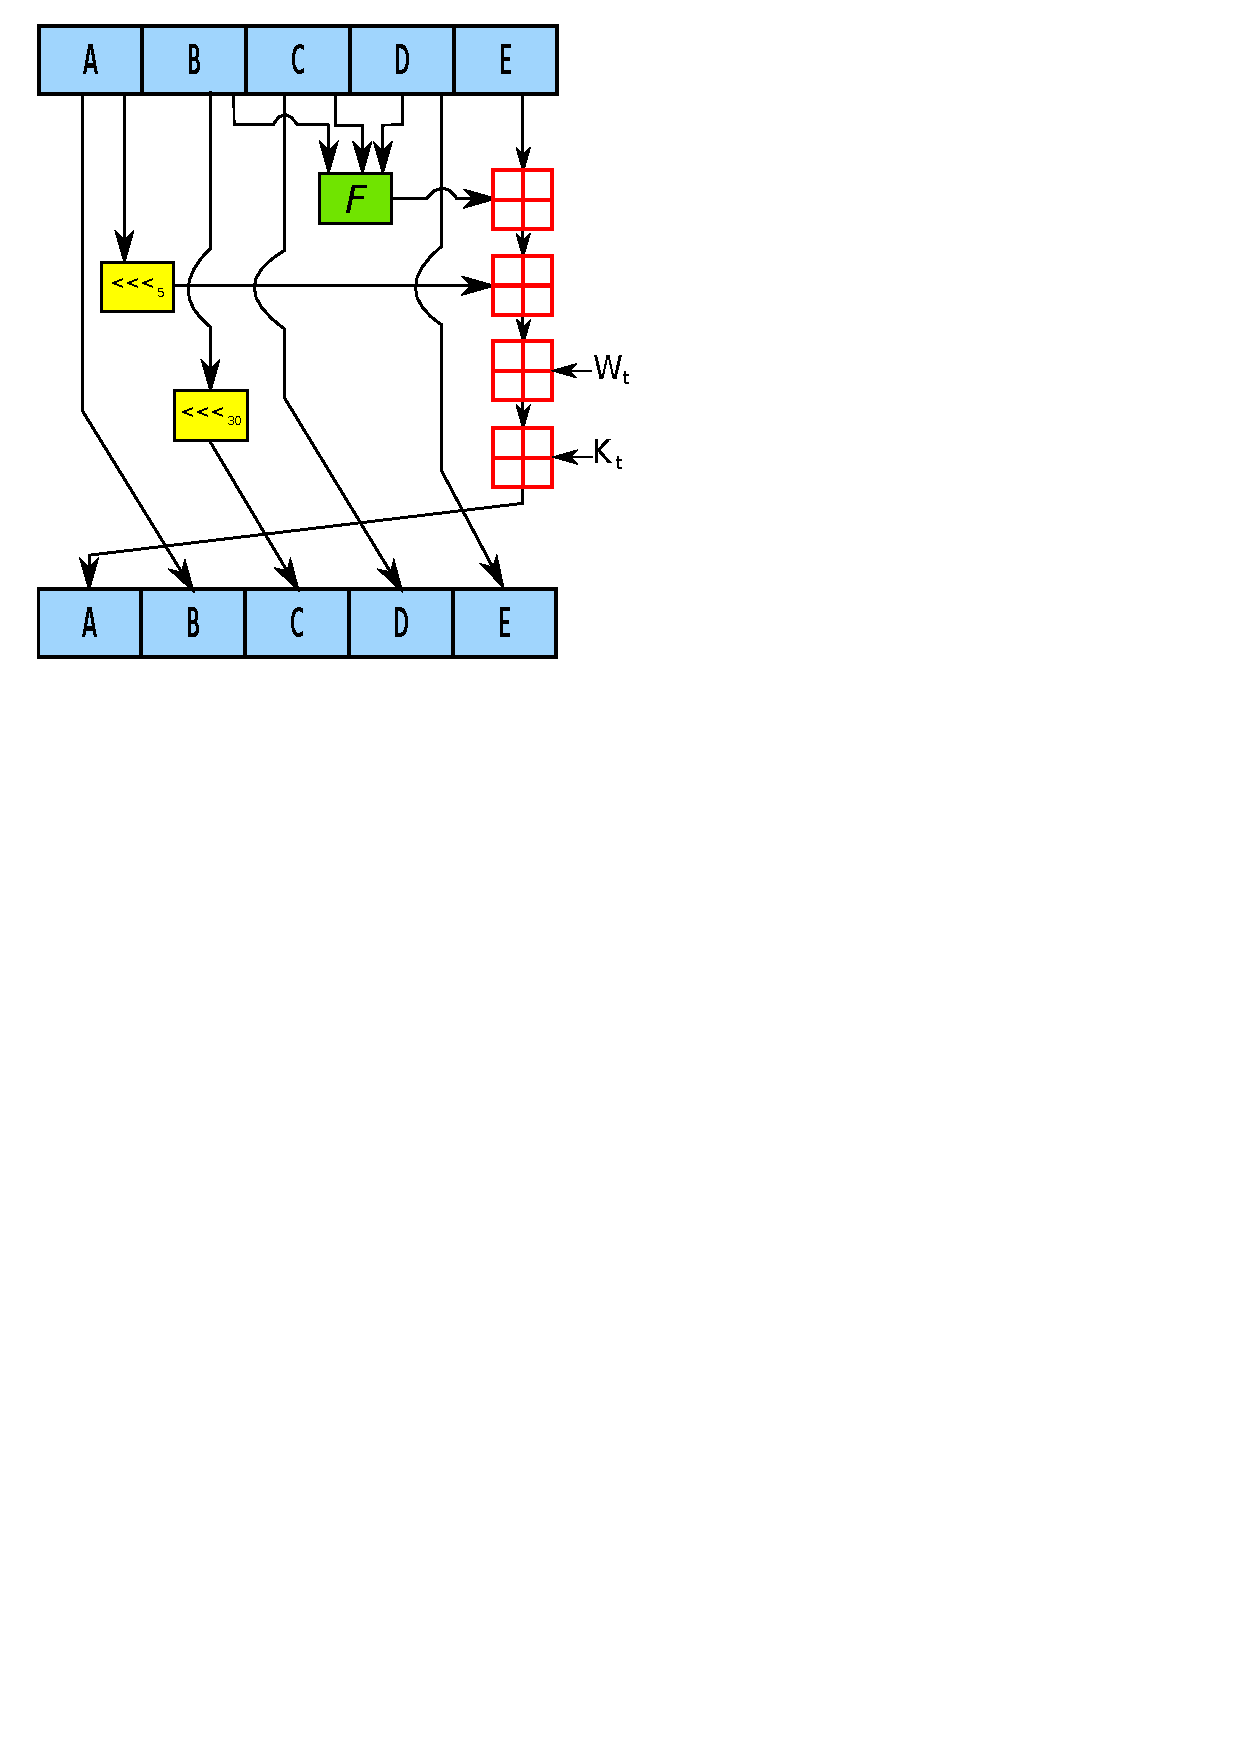
\includegraphics[width=40mm]{pic/SHA1}
\end{center}
\end{figure}
\column{.5\textwidth}
MD5:
\begin{figure}
\begin{center}
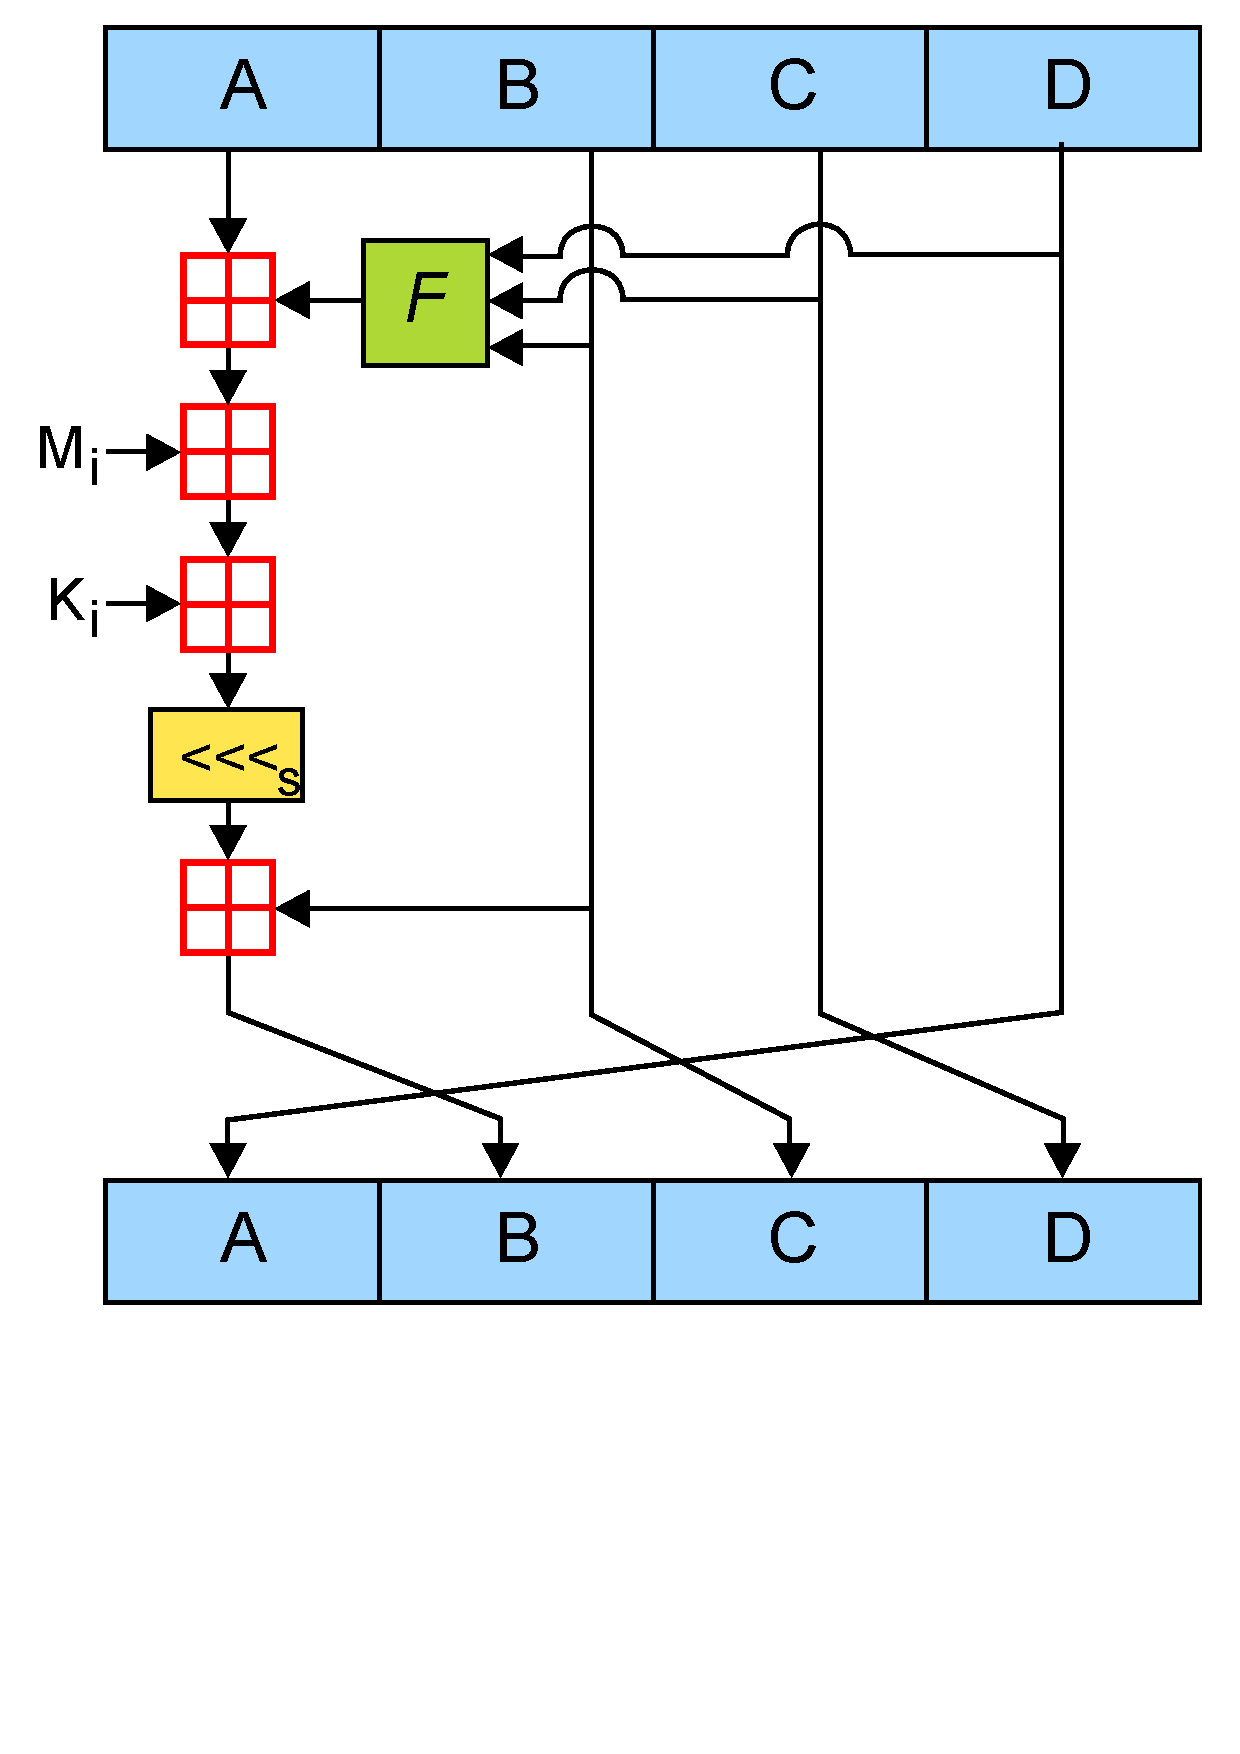
\includegraphics[width=40mm]{pic/MD5}
\end{center}
\end{figure}
\end{columns}
$A, B, C, D$ and $E$ are 32-bit words of the state;
$F$ is a nonlinear function that varies;
$\lll n$ denotes a left bit rotation by $n$ places;
$W_t$/$M_t$ is the expanded message word of round $t$;
$K_t$ is the round constant of round $t$;
$\boxplus$ denotes addition modulo $2^{32}$.
\begin{itemize}
\item Finding a collision in 128-bit MD5 requires time $2^{20.96}$. 
\item Finding a collision in 160-bit SHA-1 requires time $2^{51}$.
\end{itemize}
\end{frame}
\section{HMAC}
%\begin{frame}\frametitle{Nested MAC (NMAC)}
%\begin{figure}
%\begin{center}
%\begin{tikzpicture}[cf/.style={trapezium left angle=65, trapezium right angle=90, minimum height=1cm,minimum width=1cm,trapezium, rounded corners=1ex,shape border rotate=270, draw}]
\foreach \i in {1,2,...,5} {
\ifnum \i = 3
\node (h\i) at ($\i*(1.5cm,0)$) [trapezium left angle=65, trapezium right angle=90, minimum height=1cm,minimum width=1cm,trapezium, rounded corners=1ex,shape border rotate=270] {$\cdots$};
\else
\node (h\i) at ($\i*(1.5cm,0)$) [cf] {$h^s$};
\fi
}
\foreach \i/\j in {1/2,2/3,3/4} {
\ifnum \i = 3
\node (x\i) at ($\i*(1.5cm,0)+(0,1.5cm)$) [minimum height=0.6cm, minimum width=1.5cm] {$\cdots$};
\else
\node (x\i) at ($\i*(1.5cm,0)+(0,1.5cm)$) [minimum height=0.6cm, minimum width=1.5cm,draw] {$m_{\i}$};
\draw[-latex] (x\i) -- (h\i);
\fi
\draw[-latex] (h\i) -- (h\j);
}
\node (x4) at ($4*(1.5cm,0)+(0,1.5cm)$) [minimum height=0.6cm, minimum width=1.5cm] {$|m|$};
\draw[-latex] (x4) -- (h4);
\node (x5) at ($5*(1.5cm,0)+(0,1.5cm)$) [minimum height=0.6cm, minimum width=1.5cm] {$k_1$};
\draw[-latex] (x5) -- (h5);
\draw[-latex] (h4) -- (h5);

\node (iv) at (0,0) {$k_2$};
\node (hs) at (9cm,0) {$t$};
\draw[-latex] (iv) -- (h1);
\draw[-latex] (h5) -- (hs);
\end{tikzpicture}
%\end{center}
%\end{figure}
%\begin{construction}
%$(\widetilde{\mathsf{Gen}}, h)$ is a fixed-length CRHF. $(\widetilde{\mathsf{Gen}}, H)$ is Merkle-Damg\r{a}rd transform. NMAC:
%\begin{itemize}
%\item $\mathsf{Gen}(1^n)$: Output $(s, k_1, k_2)$. $s \gets \widetilde{\mathsf{Gen}}, k_1,k_2 \gets \{0,1\}^n$ \emph{u.a.r}.
%\item $\mathsf{Mac}_{s,k_1,k_2}(m)$: $t_i := h_{k_1}^s(H_{k_2}^s(m))$. $h_{k}^s \overset{\mathsf{def}}{=} h^s(k\|x)$.\\
%$H^s_{k_2}$ is \emph{inner} function; $h^s_{k_1}$ is \emph{outer} function.
%\item $\mathsf{Vrfy}_{s,k_1,k_2}(m,t)$: $1 \iff t \overset{?}{=} \mathsf{Mac}_{s,k_1,k_2}(m)$.
%\end{itemize}
%\end{construction}
%\end{frame}
%\begin{frame}\frametitle{Security of NMAC}
%\begin{theorem}
%If $(\widetilde{\mathsf{Gen}}, h)$ is CRHF and yields a secure MAC, then NMAC is secure. (existentially unforgeable under an adaptive CMA for arbitrary-length messages)
%\end{theorem}
%\begin{itemize}
%\item $k_2$ is not needed once $(\widetilde{\mathsf{Gen}}, h)$ is CRHF.
%\begin{itemize}
%\item \textbf{Weak collision resistance}: It is hard to find $(x, x'), x' \ne x$ such that $H^s_{k_2}(x) = H^s_{k_2}(x')$.
%\item $H_s^{k_2}(x)$ is hidden by $h_s^{k_1}(H_s^{k_2}(x))$.
%\item \textbf{Disadvantage}: $IV$ of $H$ must be modified.
%\end{itemize}
%\end{itemize}
%\end{frame}
\begin{frame}\frametitle{Hash-based MAC (HMAC)}
\begin{figure}
\begin{center}
\begin{tikzpicture}[cf/.style={trapezium left angle=65, trapezium right angle=90, minimum height=1cm,minimum width=1cm,trapezium, rounded corners=1ex,shape border rotate=270, draw}]
\foreach \i in {1,2,...,6} {
\ifnum \i = 3
\node (h\i) at ($\i*(1.5cm,0)$) [trapezium left angle=65, trapezium right angle=90, minimum height=1cm,minimum width=1cm,trapezium, rounded corners=1ex,shape border rotate=270] {$\cdots$};
\else
\node (h\i) at ($\i*(1.5cm,0)$) [cf] {$h^s$};
\fi
}
\foreach \i/\j in {1/2,2/3,3/4,4/5,5/6} {
\ifnum \i = 3
\node (x\i) at ($\i*(1.5cm,0)+(0,1.5cm)$) [minimum height=0.6cm, minimum width=1.5cm] {$\cdots$};
\else
\ifnum \i = 4
\node (x\i) at ($\i*(1.5cm,0)+(0,1.5cm)$) [minimum height=0.6cm, minimum width=1.5cm] {$|m|$};
\else
\ifnum \i = 5
\node (x\i) at ($\i*(1.5cm,0)+(0.9cm,1.5cm)$) [minimum height=0.6cm, minimum width=1.5cm] {$k\oplus opad$};
\node (iv2) at ($\i*(1.5cm,0)+(-0.5cm,1.5cm)$) [minimum height=0.6cm, minimum width=1.5cm] {$IV$};
\draw [-latex] (iv2) -- (h\i);
\else
\ifnum \i = 1
\node (x\i) at ($\i*(1.5cm,0)+(0,1.5cm)$) [minimum height=0.6cm, minimum width=1.5cm] {$k\oplus ipad$};
\else
\ifnum \i = 2
\node (x\i) at ($\i*(1.5cm,0)+(0,1.5cm)$) [minimum height=0.6cm, minimum width=1.3cm,draw] {$m_{1}$};
\else
\node (x\i) at ($\i*(1.5cm,0)+(0,1.5cm)$) [minimum height=0.6cm, minimum width=1.5cm,draw] {$k\oplus opad$};
\fi
\fi
\fi
\fi
\draw[-latex] (x\i) -- (h\i);
\fi
\ifnum \i = 4 
\draw[-latex] (h4) -| +(0.75cm,-0.7) -- +(2.1cm,-0.7) |- ($(h6.west)+(0,-0.1cm)$);
\else
\ifnum \i = 5
\draw[-latex] ($(h5.east)+(0,0.3cm)$) -- ($(h6.west)+(0,0.3cm)$);
\else 
\draw[-latex] (h\i) -- (h\j);
\fi
\fi
}
\node (iv) at (0.2cm,0) {$IV$};
\node (hs) at (10.1cm,0) {$t$};
\draw[-latex] (iv) -- (h1);
\draw[-latex] (h6) -- (hs);
\end{tikzpicture}
\end{center}
\end{figure}
\begin{construction}
$(\widetilde{\mathsf{Gen}}, h)$ is a fixed-length CRHF. $(\widetilde{\mathsf{Gen}}, H)$ is the Merkle-Damg\r{a}rd transform.
$IV$, $\mathsf{opad}$ (0x36), $\mathsf{ipad}$ (0x5C) are fixed constants of length $n$.
HMAC:
\begin{itemize}
\item $\mathsf{Gen}(1^n)$: Output $(s, k)$. $s \gets \widetilde{\mathsf{Gen}}, k \gets \{0,1\}^n$ \emph{u.a.r}.
\item $\mathsf{Mac}_{s,k}(m)$: $t := H_{IV}^s\Big((k \oplus \mathsf{opad}) \| H_{IV}^s\big((k \oplus \mathsf{ipad}) \| m\big)\Big)$.
\item $\mathsf{Vrfy}_{s,k}(m,t)$: $1 \iff t \overset{?}{=} \mathsf{Mac}_{s,k}(m)$.
\end{itemize}
\end{construction}
\end{frame}
\begin{frame}\frametitle{Security of HMAC}
\begin{theorem}
\[ G(k) \overset{\text{def}}{=} h^s(IV\| (k\oplus \mathsf{opad})) \| 
h^s(IV\| (k\oplus \mathsf{ipad})) = k_1\| k_2.
\]
$(\widetilde{\mathsf{Gen}}, h)$ is CRHF. If $G$ is a PRG, then HMAC is secure.
\end{theorem}
\begin{itemize}
\item HMAC is an industry standard (RFC2104)
\item HMAC is faster than CBC-MAC
\item Before HMAC, a common mistake was to use $H^s(k\| x)$
\item \alert{Verification timing attacks: (Keyczar crypto library (Python))} \\
def Verify(key, msg, sig\underline{\ }bytes): \\
$\qquad$ return HMAC(key, msg) == sig\underline{\ }bytes \\
The problem:  implemented as a byte-by-byte comparison
\item \alert{\emph{Don't implement it yourself.}}
\end{itemize}
\end{frame}
\begin{frame}\frametitle{Summary}
\begin{itemize}
\item adaptive CMA, replay attack, birthday attack. 
\item existential unforgeability, collision resistance.
\item CBC-MAC, CRHF, Merkle-Damg\r{a}rd transform, NMAC, HMAC. 
\end{itemize}
\end{frame}
\end{document}